\documentclass{sig-alternate}

\usepackage{amsmath}
%\usepackage{amsthm}
\usepackage{listings}
\usepackage{tikz}
\usepackage{subfigure}
\usepackage{multirow}
\usepackage{pgfplots}
\usepackage{booktabs}
\usepackage{dcolumn}
\usepackage{cancel}
\usepackage{graphics}
\usepackage{url}

\newcommand{\infrule}[2]{\displaystyle\frac{\displaystyle\strut{#1}}{\displaystyle\strut {#2}}}
\newcommand{\deref}{\ast}
\newcommand{\rread}[1]{\mbox{\em Read}(#1)}
\newcommand{\rwrite}[1]{\mbox{\em Write}(#1)}
\newcommand{\lca}[2]{#1 \sqcup #2}
\newcommand{\rleq}{\leq}
\newcommand{\interval}[1]{\mbox{\em interval}(#1)}
\newcommand{\context}[1]{\mbox{\em context}(#1)}
\newtheorem{theorem}{Theorem} 
\newtheorem{lemma}[theorem]{Lemma}

\setlength{\pdfpagewidth}{8.5in}
\setlength{\pdfpageheight}{11in}

\begin{document}

\title{High-Performance Language Primitives for Distributed Architectures using Asynchronous Events}
\numberofauthors{3}
\author{
\alignauthor Sean Treichler\\
             \affaddr{Stanford University} \\
             \email{sjt@cs.stanford.edu}
\alignauthor Michael Bauer \\
             \affaddr{Stanford University} \\
             \email{mebauer@cs.stanford.edu}
\alignauthor Alex Aiken \\
             \affaddr{Stanford University} \\
             \email{aiken@cs.stanford.edu}
}
\maketitle

\begin{abstract}
%The limit is 12 pages, including bibliography and appendices.
%Deadlines:
%\begin{tabular}{ll}
%Abstract deadline & July 16, 2012 3pm PDT \\
%Paper deadline & July 23, 2012 3pm PDT \\
%Author response & around October 15, 2012 \\
%Author notification & November 9, 2012
%\end{tabular}
We present a low-level runtime interface for current highly distributed, heterogeneous
parallel machines that provides a fully asynchronous 
programming model, allowing all types of runtime actions, including synchronization,
to be non-blocking.  Our interface includes mechanisms for the creation and movement
of data through the memory hierarchy as well as {\em deferred locks}, a novel synchronization primitive.
Asynchrony is exposed by the interface using a distributed event system.  All
operations return an event to be triggered when the operation completes.  Events
can be chained together and used to capture dependences between operations.

We describe an implementation of our interface capable of running on
a large supercomputer with both CPU and GPU processors and a high speed interconnect.
We employ several micro-benchmarks to show that our implementation approaches
the performance limits of the underlying hardware.
We also demonstrate that the interface is sufficiently powerful to serve as the foundation 
of an advanced parallel programming system.  We measure the performance of three real-world applications
that use our system on the Keeneland supercomputer.
\end{abstract}

%\section{Proof Outline}

\begin{itemize}

\item A logical region $L$ is a set of abstract memory locations $a_i, a_j, ... \in A$.

\item A coloring function $c : A \rightarrow C$ is a function from abstract memory locations to ``colors''.

\item A partitioning $P_{L,c} : C \rightarrow 2^A$ of a region $L$ with a coloring function $c$ is a function from a color to a subregion of L, satisfying:

\begin{itemize}

\item $\forall L,c,i,a . a \in L \wedge c(a) = i \leftrightarrow a \in P_{L,c}(i)$

\item $\forall L,c,i_1,i_2 . i_1 \neq i_2 \rightarrow P_{L,c}(i_1) * P_{L,c}(i_2)$

\end{itemize}

\item A static effect $E$ is a set of tuples $\langle L, op \rangle$ where $op \in \{ read, write \} \cup \{ reduce_f : f \text{is a reduction function} \}$.

\item Physical memory locations are represented by the set $m_1, m_2, ... \in M$, along with a mapping function $\alpha : M \rightarrow A$ that describes which abstract location a physical memory location corresponds to.

\item A dynamic trace $D = \langle \hat E, \hat O \rangle$ is a directed acyclic graph whose nodes $\hat E$ are actual memory operations $\langle m, op \rangle$ and edges $\hat O$ describe a partial ordering $\hat e_1 \prec \hat e_2$ of those memoory operations.  (Hmm...  Need notation that makes it clear that the same memory operation can be performed on the same memory address multiple times.)

\item Soundness of effects: If $\vdash t : ^ET$ then the mapping function $\alpha$ and dynamic trace $D = \langle \hat E, \hat O \rangle$ that results from evaluating $t$ have the following properties:

\begin{itemize}

\item $\forall m . \langle m, read \rangle \in \hat E \rightarrow \exists L . \alpha(m) \in L \wedge \langle L, read \rangle \in E$

\item $\forall m . \langle m, write \rangle \in \hat E \rightarrow \exists L . \alpha(m) \in L \wedge \langle L, write \rangle \in E$

\item $\forall m, f . \langle m, reduce_f \rangle \in \hat E \rightarrow ( \exists L . \alpha(m) \in L \wedge \langle L, reduce_f \rangle \in E ) \vee ( \exists L_1, L_2 . \alpha(m) \in L_1 \wedge \langle L_1, read \rangle \in E \wedge \alpha(m) \in L_2 \wedge \langle L_2, write \rangle \in E )$

\end{itemize}

\item Two dynamic subtraces $D_1 = \langle \hat E_1, \hat O_1 \rangle$, and $D_2 = \langle \hat E_2, \hat O_2 \rangle$ are ``memory ordered'' (written $D_1 \prec_D D_2$) within a larger trace $D = \langle \hat E_1 \cup \hat E_2 \cup \hat E', \hat O_1 \cup \hat O_2 \cup \hat O' \rangle$ if $D_2$ sees all the results of $D_1$'s memory operations and $D_1$ sees none of the results of $D_2$'s memory operations:

\begin{tabular}{l@{}l@{}l}
$D_1 \prec_D D_2 \leftrightarrow \forall$ & $\hat e_1 = \langle m_1, op_1 \rangle \in \hat E_1,$ \\
& $\hat e_2 = \langle m_2, op_2 \rangle \in \hat E_2 . \big($ & $m_1 \neq m_2 \vee$  \\
&& $( op_1 = read \wedge op_2 = read ) \vee$ \\
&& $( op_1 = reduce_f \wedge op_2 = reduce_f ) \vee$ \\
&& $( \hat e_1 \prec \hat e_2 \in \hat O' ) \big)$
\end{tabular}

\item Note that if $D_1$ and $D_2$ have no memory addresses in common, then you have $D_1 \prec_D D_2$ and $D_2 \prec_D D_1$ for all D.  Maybe $\prec$ is the wrong symbol to use?

\item Tasks are annotated with a coherence requirements $H_{excl}, H_{atom} \subseteq A$.  The default annotation is $H_{excl} = \bigcup_{\langle L, op \rangle \in E} L, H_{atom} = \emptyset$.

\item The runtime enforces an execution order $\prec_E$ between two tasks $S_1$ and $S_2$ as follows:

\begin{itemize}

\item Strict ordering: when the two tasks have exclusive coherence requirements on two regions that can't be proven disjoint (i.e. $\not\vdash H_{excl_1} * H_{excl_2}$), we enforce $S_1 \prec_E S_2$.

\item Serializability: when the two tasks have atomic coherence requirements on two regions that can't be proven disjoint, we enforce $S_1 \prec_E S_2 \vee S_2 \prec_E S_1$.

\end{itemize}

\item Execution order is stronger than memory order: $(S_1 \prec_E S_2) \rightarrow ( \forall \hat e_1 \in \hat E_1, \hat e_2 \in \hat E_2 . \hat e_1 \prec \hat e_2 ) \rightarrow (\forall D. D_1 \prec_D D_2)$.

\item Coherence of sibling tasks:  If sibling tasks $S_1$ and $S_2$ are program ordered (i.e. $S_1 \prec_P S_2$) within their parent task:

\begin{itemize}

\item Overlap in exclusivity requirements guarantees memory ordering: $H_{excl_1} \cap H_{excl_2} \neq \emptyset \rightarrow D_1 \prec_D D_2$.  (If $\vdash (E_1 \cap H_{excl_1}) * (E_2 \cap H_{excl_2})$, soundness of effects guarantees disjointness of memory addresses and therefore memory ordering.  If not, the runtime enforces execution order and therefore memory ordering.)

\item Overlap in atomic requirements guarantees serializability: $H_{atom_1} \cap H_{atom_2} \neq \emptyset \rightarrow D_1 \prec_D D_2 \vee D_2 \prec_D D_1$.  (Parallels proof above.)

\end{itemize}

\end{itemize}



\section{Introduction}
\label{sec:intro}

Machine architecture, particularly at the high
performance end of the spectrum, has recently undergone a revolution.  The
latest supercomputers are now composed of heterogeneous processors
and deep memory hierarchies.  Current programming systems for these
machines have elaborate features for describing parallelism, but 
few abstractions for describing the organization of data.  However, as 
distributed memory machines increase in complexity,
reasoning about the organization of program data will be imperative
for supporting the management of parallelism and the movement of data
through the memory hierarchy.

%Consequently, the burden of managing
%the correctness of parallel computations and movement of data
%through the memory hierarchy is placed on the programmer.

%However,
%these systems relegate to the programmer the responsibility for:
%\begin{itemize}
%\item the correctness of their parallel declarations
%\item the movement and placement of data in the memory hierarchy
%\end{itemize}
%Coupled with the complexity of these machines, this places a heavy
%burden on the programmer.  The reason that the programmer must bear
%this load is because current programming systems have few or no
%insights into properties of program data (e.g. locality and independence).  
%To enable more efficient programming of this class of machines we 
%need programming systems capable of reasoning both statically and dynamically
%about the structure of program data.

Previous work has explored two approaches for describing the organization of data
in distributed memory programs.
One class of work uses fully static analyses with no runtime overhead, but 
disallows potential data aliasing to make the analysis tractable, limiting expressivity.
Two recent examples, Sequoia \cite{Fatahalian06} and 
Deterministic Parallel Java (DPJ) \cite{Bocchino09}, each provide a 
mechanism to statically partition the heap.
% into a tree of collections of data.
The two designs are different in many aspects, but agree that there is
a single tree-shaped partitioning of data that must be checked statically 
(see Section~\ref{sec:related}).  The second approach permits data
aliasing, allowing greater expressivity, but uses fully dynamic analyses of
program execution to detect aliasing and guarantee correct results.
This approach incurs significant runtime overhead and requires 
centralized control logic that is difficult to scale to distributed 
memory machines; examples include transactional memory \cite{Harris05} 
and thread-level speculation \cite{Steffan00}.

Our own experience writing high-performance applications
using the current industry standard mix of MPI, shared-memory
threads, and CUDA has taught us that a
single, static data partitioning is often insufficient.  In many cases, the
best way to partition data is often a function of the data
itself---i.e., the partitions must be dynamically computed and cannot be statically described.
Furthermore, applications often need multiple, simultaneous partitions of
the same data, which introduces aliasing.

In this work, we present the static and dynamic semantics of Legion \cite{Legion12},
a parallel programming model that supports multiple, dynamic data partitions and is
able to efficiently reason about potential aliasing.
Legion's {\em logical regions} are an abstraction capturing {\em locality} 
(data that will be used together, and therefore should be colocated) 
and {\em independence} (disjoint data that may be operated on in parallel).  
Logical regions have properties that allow programmers to communicate information
about the structure of program data to the Legion implementation:
\begin{itemize}
\item  logical regions are first-class values in Legion
and may be dynamically allocated and stored in data structures;

\item logical regions can be dynamically {\em partitioned} into {\em subregions}; 
the programmer can express arbitrary partitions of regions;

\item  a logical region may be dynamically partitioned in multiple different ways;
subregions from multiple partitions may include the same data, introducing 
aliasing\footnote{Thus
  the term {\em logical} regions: language-level regions
  name sets of data but do not imply a physical layout or placement in
  the memory hierarchy. A separate system of {\em physical regions} at
  runtime holds copies of data in the language-level logical regions
  \cite{Legion12}.}.

%\item {\em privilege} and {\em coherence} properties that
%describe how a logical region's data may be used by computations (explained below).
\end{itemize}

%Both dynamically computed partitions
%and simultaneous partitions of the same data introduce the possibility
%of {\em aliasing}---distinct regions may have overlapping data.

While data in Legion is organized in a hierarchy of logical regions,
computation is organized in a hierarchy of tasks.  Logical regions and tasks interact
through a system of {\em privileges} that specify which operations (read, write, or reduce)
a task (or any of its subtasks) may perform on each logical region argument.  
%Tasks can only access logical regions for which they 
%possess privileges.  
%Tasks acquire privileges from their calling task
%or by creating new logical regions.  A key restriction is that 
%a sub-task can only be passed a subset of the privileges of its parent task.  

%Through multiple partitions of a logical region, a given datum may
%belong to multiple different regions.  

To support additional parallelism in the presence of aliased data,
Legion provides {\em coherence} modes at the granularity of regions,
which allow relaxed constraints on task execution order, even
in cases where tasks access the same region.  The programmer may
specify that tasks conflicting on a region run in
program order (the default), {\em atomically} with respect to each
other, or even {\em simultaneously} if the application has alternative
methods for ensuring determinism or can tolerate non-deterministic
behavior in that region.

%To guarantee the safety and correctness of programs, Legion relies on
%a combination of static and dynamic analysis based on the privilege
%and coherence systems.  
%To efficiently guarantee the safety and
%correctness of programs using first-class regions,
%privilege and coherence properties in the presence of arbitrary region
%aliasing, Legion relies on a combination of static and
%dynamic checks.  
The critical feature in Legion that makes static analysis tractable
and dynamic analysis efficient in the presence of potential aliasing is logical regions.
Alias analysis is a very hard static analysis problem, but is both easy and
inexpensive if done dynamically at the granularity of logical regions instead
of individual memory locations; similarly
checks on individual memory accesses are expensive if done dynamically, but
cheap if done statically within the context of local logical region privileges.
%A key theme that runs through the design is that 
%alias analysis is a very hard static analysis problem, but is both easy and
%inexpensive if done dynamically at the granularity of regions instead of individual
%heap locations, while checks that must be done on individual values are only
%cheap if done statically.  
Explicating and evaluating the design of Legion's
static and dynamic semantics is the topic of this paper, 
%and its implications are the topics of this paper,
which we present as a series of contributions:
\begin{itemize}
\item We present a type system for {\em Core Legion} programs that statically
  verifies the safety of individual pointers and region
  privileges at task call boundaries (Section~\ref{subsec:coretypes}).
%  A subtle issue arises in checking privileges when regions are
%  stored in and later retrieved from heap data structures.  The type
%  system provides enough static information that the Legion runtime
%  can leverage its dynamic information about region aliasing to
%  perform dynamic privilege checks guaranteeing safety.

\item We present a novel parallel operational semantics for Core Legion.
 This semantics is compositional,
  hierarchical, and asynchronous, reflecting the way such programs
  actually execute on the hardware.  The semantics also
  models conflicting memory operations between tasks in cases of relaxed
  coherence, making explicit the boundary between deterministic and
  possible non-deterministic behavior (Section~\ref{subsec:opsemantics}).

\item We prove the soundness of Legion's static type and privilege system (Section~\ref{sec:soundness}).


\item We use soundness of the type system to prove the soundness of
  Legion's region coherence modes (Section~\ref{sec:coherence}).


\item Again using the soundness of the type system,  we show that if expressions $e_1$ and $e_2$ 
are {\em non-interfering} (can be executed in parallel), then subexpressions
$e_1'$ of $e_1$ and $e_2'$ of $e_2$ are also non-interfering (Section~\ref{sec:scheduling}).  
This result is the basis
for a hierarchical, distributed scheduler in the Legion implementation which is crucial for high performance
on the target class of machines.
%  any form of centralized scheduling would be a bottleneck because of the
%large communication latencies in the target class of machines.
%; on the target class of machines, any centralized
%scheduler would be a serious bottleneck.

\item We give experimental evidence that supports the Legion design choices.  On three
  real-world applications, we show that dynamic region pointer checks
  would be expensive, justifying checking this aspect of the type
  system statically.  We also show that the cost of region aliasing
  checks is low, showing that an expressive and dynamic
  language with aliasing is compatible with both high
  performance and safety (Section~\ref{sec:evaluation}).

\end{itemize}






%The crucial aspect of this result is that the tasks $t_1$ and $t_2$ only 
%need be non-interfering instead of non-aliased.  Thus, through a combination
%of static and dynamic analysis, our privilge type system and coherence system
%enable us to implement a hierarchical, distributed scheduling algorithm even
%in the presence of aliasing introduced by the need for dynamic descriptions of
%data via first-class logical regions.  
%All of this is possible only because
%our programming system supports an abstraction for understanding the structure
%of program data.



%The important difference between Legion and the more static approaches
%is that Legion allows region aliasing, but does so in a structured way that minimizes
%runtime overheads.  
%The key observation is that static alias analysis is hard, but dynamic 
%alias analysis is very easy and relatively cheap when done at the granularity 
%of regions instead of individual heap locations.  
%Thus, Legion falls between fully static systems, such as
%Sequoia and DPJ, and fully dynamic approaches such as transactional
%memory.  
%Legion still has a significant static component; in
%particular, the required privileges for function calls
%and region
%pointer dereferences are checked statically.  The dynamic alias checks
%for independence are done at the granularity of regions and one check 
%on a region
%often serves to prove the independence of many subsequent uses of that region.
%In contrast, because transactional memory has no mechanism
%for grouping heap data into larger collections, it must test the
%overlap between two sets of data on each individual memory location, which is
%significantly more expensive.



%which makes it difficult 
%to statically determine which computations can be run in parallel.  
%One approach is to outlaw aliasing which allows for a static analysis
%to discover all available parallelism and schedule it entirely at
%compile-time, avoiding any runtime overhead.  Languages such as
%Sequoia and DPJ take this approach and allow only a single static partition of any region 
%to eliminate region aliasing, at some cost in expressiveness.



%While many programming systems for
%these machines have intricate features for describing parallelism,
%few have any abstractions for capturing properties of a program's data (e.g.
%independence and locality).  Understanding the structure of a program's data
%is critical for allowing programming systems to validate/discover
%parallelism or support placement of data in the memory hierarchy.  
%The few programming systems that do support data abstraction 
%features\cite{Fatahalian06,Bocchino09} permit only
%statically analyzable abstractions which restrict expressivity.  We
%present a type system for Legion\cite{Legion12}, a programming model
%that permits both static and dynamic descriptions of the structure of 
%program data.  Despite the dual nature of Legion, our type system allows us 
%to statically prove several useful properties about the structure and usage 
%of data in Legion programs.  We show how to leverage these properties 
%to enable a scalable, hierarchical scheduling algorithm based on a 
%dynamic analysis of program data.

%complex hierarchies of many different
%kinds of computing technologies: networks of nodes at the top level,
%multiple chips per node, multiple cores within a chip, and, 
%recently, multiple accelerators (usually GPUs) per node, which 
%can themselves be further decomposed.  We present the operational and static
%semantics of Legion\cite{Legion12}, a programming model targeted at providing an
%appropriate level of abstraction for programming such machines, one
%that is both sufficiently high-level to be portable while still
%exposing aspects that are crucial to performance. 

%The primary abstraction for capturing the structure of data in Legion is {\em logical regions}. Logical
%regions express {\em locality} (data that will be used together, and therefore should be colocated) 
%and {\em independence} (disjoint data that may be operated on in parallel).
%Legion programs organize data into a forest of logical regions.  Logical regions can be
%recursively partitioned into sub-regions.  

%In Legion data is organized in a hierarchy of {\em regions}
%and subregions while computation is organized in a hierarchy of {\em
%tasks} and subtasks operating on regions.  Regions and tasks interact
%through a static system of {\em region privileges} specifying 
%operations a task may perform on a region argument (read,
%write, or reduce) and  {\em region coherence} annotations that
%express what other tasks may do concurrently with
%the region (exclusive, atomic, or simultaneous).  We prove the
%soundness of the privileges and coherence system and use these two
%results to prove a third result: if two {\em siblings} (tasks that
%have the same immediate parent task) $t_1$ and $t_2$ are 
%{\em non-interfering} (have no ordering requirements for correctness), 
%then the any descendant of $t_1$ in the task hierarchy is non-interfering
%with any descendant of $t_2$.  This theorem is the basis for correct distributed
%task scheduling in a Legion implementation, which is crucial for
%performance; a centralized scheduler would be a bottleneck
%because of the large communication latencies in the target
%class of machines.


% Putting this here so that we can get the code in a good place
% Moving this to the circuit example section since it fits better there
% and some of this is redundant
%Legion's execution model is that by default, a program's semantics is
%its meaning as a sequential program, which we refer to as the {\em
%program order} execution.  While the
%implementation is not our focus here, if two functions use
%disjoint data (because all of the regions they use are disjoint), then
%Legion may execute them simultaneously.  Also like DPJ,
%Legion has a system of {\em privileges} ({\em read}, {\em write}, and
%{\em reduce}) on regions and an orthogonal system of region {\em
%coherence} modes ({\em excl}, {\em atomic}, and {\em simultaneous})
%that increase the number of situations in which functions can be
%executed in parallel.

%The rest of the paper is organized as follows.
%We begin in Section~\ref{sec:example} with an example program that illustrates
%a typical style of programming in Legion and motivates the need for multiple, dynamically computed partitions of
%a region that introduce aliased data.  We define Core Legion, a small language suitable 
%for our formal development, in Section~\ref{sec:legioncore}.
%Finally, Section~\ref{sec:related} discusses the most closely related work and
%Section~\ref{sect:conclusion} concludes.


  












\section{Programming Interface}
\label{sec:interface}
The target set of clients for our interface are higher-level language
compilers and runtimes such as Legion\cite{Legion12} as well as 
advanced systems programmers.  This class of clients expect total control
over the underlying hardware and transparent performance from an
implementation.  To support these demands we have designed our interface
to be as low-level as possible.  In many cases we have chosen to trade-off
ease of programmability for performance.  We eschewed any features that would
automatically be performed without being directed by the client.
Our goal in the design of this interface is to provide a set of low-level,
high-performance primitives that are asynchronous and composable.

Our interface is shown in Figure~\ref{fig:runtimeapi} and organizes functionality into objects.  We describe
these objects in six parts: {\em events} for composing operations 
(Section~\ref{subsec:events}), {\em processors} for parallel computation 
(\ref{subsec:procs}), {\em barriers} for producer/consumer coordination (\ref{subsec:barriers}),
{\em deferred locks} for more general synchronization
(\ref{subsec:locks}), {\em physical regions} for data layout and movement
(\ref{subsec:phyreg}), and a {\em machine} object for introspection of the underlying
hardware (\ref{subsec:machmodel}).  In all cases (except for the
machine object which is a static singleton), instances of the objects
are light-weight {\em handles} that provide a unique name for an underlying
implementation object.
Every handle is valid everywhere in the system, allowing handles to be freely copied,
passed as arguments to other tasks, or stored in the heap
without having to reason about the distributed nature of the system.
%%   Multiple copies of handles are permitted and handles can be 
%% passed by value.  Furthermore, every handle is valid everywhere in the system.  
%% This property allows a client to pass handles by value between computations 
%% without having to reason about the distributed nature of the system.
%We describe how we support this property in more detail in 
%Section~\ref{sec:impl}.

\lstset{
  captionpos=b,
  language=C++,
  basicstyle=\scriptsize,
  numbers=left,
  numberstyle=\tiny,
  columns=fullflexible,
  stepnumber=1,
  escapechar=\#,
  keepspaces=true,
  belowskip=-10pt,
  literate={<}{{$\langle$}}1 {>}{{$\rangle$}}1,
  %morekeywords={region,coloring,partition,spawn,disjoint,aliased},
  %deletekeywords=float,
}

\subsection{Events}
\label{subsec:events}
Events are the primary mechanism for describing dependences between operations in our system.
Lines 1-13 of Figure~\ref{fig:runtimeapi} show the interface for events.  An instance of the {\tt Event} type 
names a unique event in the system.  {\tt NO\_EVENT} (line 3)
is a special instance
of an event that by definition has always triggered.  The event interface
supports testing whether an event has triggered (line 5) and waiting on
an event to trigger (line 6).  While these methods can be useful, the preferred
use of events is passing them as preconditions for other operations.  The client can use the
{\tt merge\_events} call (line 7) to create an event that triggers only when every
event in a given set of events has triggered.  A code example using events follows in
Section~\ref{subsec:procs}.
%corresponding to the conjunction of a set of events.

In most cases events are created as the result of other
operations and the implementation is responsible for triggering these events.  Clients
can also create a {\tt UserEvent} (line 10) that is triggered explicitly by the client,
and may be used as precondition like any other event.

%Although user events and barriers are created and triggered differently,
%operations that express dependences on Events can transparently use
%UserEvents or Barriers as well.

%%   Users can also create another
%% type of event called a {\tt Barrier} that will require multiple arrivals before
%% the event is triggered.  The user can manage the number of arrivals that must
%% be seen as well as how many arrivals occur at a time.  Once a barrier's arrival
%% count goes to zero, the barrier will trigger.  Note that barriers in our interface
%% provide a superset of the functionality of traditional barriers since they can
%% be used in a blocking manner (via the {\tt wait} call), but are primarily used
%% asynchronously.  Lastly, since user events and barriers are sub-types of 
%% an event they can be used wherever an event is required.

\begin{figure}
\begin{lrbox}{\mylistingbox}
\begin{lstlisting}
class Event {
  const unsigned id, gen;
  static const Event NO_EVENT;

  bool has_triggered() const;
  void wait() const;
  static Event merge_events(const set<Event> &to_merge);
};

class UserEvent : public Event {
  static UserEvent create_user_event();
  void trigger() const;
};
\end{lstlisting}
\end{lrbox}
\subfigure{\usebox{\mylistingbox}} \\

\begin{lrbox}{\mylistingbox}
\begin{lstlisting}[firstnumber=14]
class Processor {
  const unsigned id;
  typedef unsigned TaskFuncID;
  typedef void (*TaskFuncPtr)(void *args,size_t arglen,Processor p);
  typedef map<TaskFuncID, TaskFuncPtr> TaskIDTable;

  enum Kind { CPU_PROC,GPU_PROC /* ... */ };
  Kind kind() const;

  Event spawn(TaskFuncID func_id,const void *args,size_t arglen, Event wait_on) const;
};
\end{lstlisting}
\end{lrbox}
\subfigure{\usebox{\mylistingbox}} \\

\begin{lrbox}{\mylistingbox}
\begin{lstlisting}[firstnumber=25]
class Barrier : public Event {
  static Barrier create_barrier(unsigned expected_arrivals);
  void alter_arrival_count(int delta) const;
  void arrive(unsigned count = 1, Event wait_for = NO_EVENT) const;
};
\end{lstlisting}
\end{lrbox}
\subfigure{\usebox{\mylistingbox}} \\

\begin{lrbox}{\mylistingbox}
\begin{lstlisting}[firstnumber=30]
class Lock {
  const unsigned id;
  Event lock(Event wait_on = NO_EVENT) const;
  void unlock(Event wait_on = NO_EVENT) const;

  static Lock create_lock(size_t payload_size = 0);
  void *payload_ptr();
  void destroy_lock();
};
\end{lstlisting}
\end{lrbox}
\subfigure{\usebox{\mylistingbox}} \\

\begin{lrbox}{\mylistingbox}
\begin{lstlisting}[firstnumber=39]
class Memory {
  const unsigned id;
  size_t size() const;
};

class RegionMetaData {
  const unsigned id;
  static const RegionMetaData NO_REGION;

  static RegionMetaData create_region(size_t num_elmts, size_t elmt_size);
  void destroy_region() const;

  RegionInstance create_instance(Memory memory) const;
  RegionInstance create_instance(Memory memory, ReductionOpID redopid) const;
  void destroy_instance(RegionInstance instance) const;
};

class RegionInstance {
  const unsigned id;

  Event copy_to(RegionInstance target, Event wait_on = NO_EVENT);
  Event reduce_to(RegionInstance target, ReductionOpID redopid, Event wait_on = NO_EVENT);
};
\end{lstlisting}
\end{lrbox}
\subfigure{\usebox{\mylistingbox}} \\

\begin{lrbox}{\mylistingbox}
\begin{lstlisting}[firstnumber=62]
class Machine {
  Machine(int *argc, char ***argv, const Processor::TaskIDTable &task_table);

  void run(Processor::TaskFuncID task_id, const void *args, size_t arglen);

  static Machine* get_machine(void);
  const set<Memory>& get_all_memories(void) const;
  const set<Processor>& get_all_processors(void) const;

  int get_proc_mem_affinity(vector<ProcMemAffinity> &result, ...);
  int get_mem_mem_affinity(vector<MemMemAffinity> &result, ...);
};
\end{lstlisting}
\end{lrbox}
\subfigure{\usebox{\mylistingbox}} \\

\caption{Runtime Interface.\label{fig:runtimeapi}}
\vspace{-4mm}
\end{figure}

\subsection{Processors}
\label{subsec:procs}
Lines 14-24 of Figure~\ref{fig:runtimeapi} show the interface for {\tt Processor} objects which allow for
the creation of parallel computations.  Processors provide a way of naming 
every computational unit in the machine.  We describe how to discover processor handles
in Section~\ref{subsec:machmodel}.  In the case of our current interface 
processors are either individual CPU cores or discrete GPUs, but this is easily modified 
to include new processor types (line 20).   Processors support a single {\tt spawn}
method (line 23) that launches a new {\em task} on that processor.
Note that because the spawn operation
is invoked on a processor handle, it is possible to launch a task on any
processor from anywhere in the system.  
The spawn call takes an optional event that must trigger before the task can begin, and
always returns an event that will trigger when the task completes.

Figure~\ref{fig:procevents} shows a simple example using 
the processor and event interface.  The {\tt diamond\_task} launches four
sub-tasks with a diamond dependence pattern.
The {\tt merge\_events} call
merges the events {\tt eb} and {\tt ec} to create the shared dependence
for the last sub-task.

\begin{figure}
\begin{lrbox}{\mylistingbox}
\begin{lstlisting}
void diamond_task(const void *args,size_t arglen,Processor p){
  Event ea = p.spawn(TASK_A,NULL,0);
  Event eb = p.spawn(TASK_B,NULL,0,ea);
  Event ec = p.spawn(TASK_C,NULL,0,ea);
  Event em = Event::merge_events(eb,ec);
  Event ed = p.spawn(TASK_D,NULL,0,em);
}
\end{lstlisting}
\end{lrbox}
\subfigure{\usebox{\mylistingbox}}\\

\centering
\scalebox{0.8}{
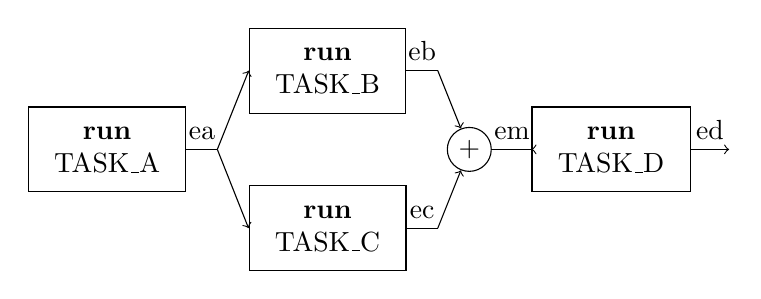
\begin{tikzpicture}
  %\path (1,3) node (t1) [shape=rectangle,draw] {run TASK\_A} -- node [right=1pt] {ea} +(0,-0.5) node[auto] {eax};
  \node (t1) at (0,0) [shape=rectangle,draw] {\begin{tabular}{c}{\bf run}\\TASK\_A\end{tabular}};
  \draw (t1) to node[auto] {ea} (1.4,0);

  \node (t2) at (2.8,1) [shape=rectangle,draw] {\begin{tabular}{c}{\bf run}\\TASK\_B\end{tabular}};
  \draw (t2) to node[auto] {eb} (4.2,1);
  \draw [->] (1.4,0) to (t2.west);

  \node (t3) at (2.8,-1) [shape=rectangle,draw] {\begin{tabular}{c}{\bf run}\\TASK\_C\end{tabular}};
  \draw (t3) to node[auto] {ec} (4.2,-1);
  \draw [->] (1.4,0) to (t3.west);

  \node (t4j) at (4.6,0) [shape=circle,inner sep=2pt,draw] {+};
  \draw (t4j) to node[auto] {em} (5.4,0);
  \draw [->] (4.2,1) to (t4j);
  \draw [->] (4.2,-1) to (t4j);

  \node (t4) at (6.4,0) [shape=rectangle,draw] {\begin{tabular}{c}{\bf run}\\TASK\_D\end{tabular}};
  \draw [->] (t4) to node[auto] {ed} (7.9,0);
  \draw [->] (5.4,0) to (t4.west);
  %
\end{tikzpicture}
}
%\vspace{-2mm}
\caption{Processor Example and Event Graph.\label{fig:procevents}}
\vspace{-4mm}
\end{figure}

\subsection{Barriers}
\label{subsec:barriers}
The common synchronization pattern in which multiple consumers are dependent on
a set of producers is supported by a {\tt Barrier} object (lines 25-29 of Figure~\ref{fig:runtimeapi}), which is similar
to a user event, but does not trigger until the expected number of {\tt arrive}
operations have occurred.  To better support
composability and asynchronous operation, our interface differs from barriers in other programming
models\cite{MPI} in three fundamental ways:
%The common synchronization pattern in which multiple consumers are dependent on a 
%(potentially different) set of producers is supported by a {\tt Barrier} object,
%which is similar to a {\tt UserEvent}, but does not trigger until the expected
%number of {\tt arrive} operations have occurred.  Barrier constructs exist in other
%programming models\cite{MPI}, but in addition to the decoupling of the waiters from
%the arrivers, our barrier interface has two further improvements to better support
%composability and asynchronous operation:
\begin{itemize} \itemsep1pt \parskip0pt \parsep0pt
\item The set of producers arriving at the barrier can be different from the set of consumers waiting on the barrier.
\item An arrival operation can be made dependent on another event, allowing a client to
express that an operation should be completed before the barrier can trigger.
\item The expected arrival count of a barrier can be dynamically modified, which we
have found useful in supporting nested parallelism in higher-level languages.
%allowing
%producer tasks to be subdivided as necessary, even after the barrier has been created.
\end{itemize}

Like user events, barriers are a sub-type of events and can therefore
be used transparently to express dependences wherever events are used.

\subsection{Deferred Locks}
\label{subsec:locks}

Events and barriers express ordering properties between operations, but 
%in many cases 
ordering is often too strict a requirement.  For many applications access to data need only be atomic and
not necessarily ordered.  Traditionally locks have been used to serialize access to
data.  However, all lock implementations that we are aware of require either blocking
or spinning, neither of which composes well with asynchronous operations.
{\em Deferred locks} are a new synchronization mechanism that allows for synchronization
without blocking or spinning.
%in an completely non-blocking environment.  

\begin{figure}
\begin{lrbox}{\mylistingbox}
\begin{lstlisting}
void lock_example(const void *args, size_t arglen, Processor p) {
  // Unpack lock, input events, target processors from arguments
  Lock needed = ...
  // Acquire lock, launch first subtask, release lock
  Event lock_event_1 = needed.lock(prev_event_1);
  Event task_event_1 = proc1.spawn(SUB, args_1, sizeof(args_1), lock_event_1);
  needed.unlock(task_event_1);
  // same for second subtask
  Event lock_event_2 = needed.lock(prev_event_2);
  Event task_event_2 = proc2.spawn(SUB, args_2, sizeof(args_2), lock_event_2);
  needed.unlock(task_event_2);
}
\end{lstlisting}
\end{lrbox}
\subfigure{\usebox{\mylistingbox}}\\

\centering
\scalebox{0.8}{
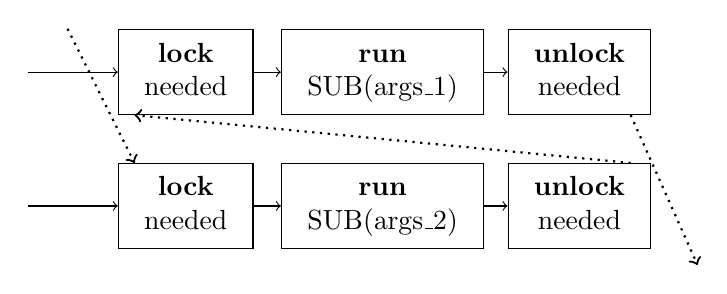
\begin{tikzpicture}
  \node (l1) at (2,1.95) [shape=rectangle,draw] {\begin{tabular}{c}{\bf lock}\\needed\end{tabular}};
  \node (t1) at (4.5,1.95) [shape=rectangle,draw] {\begin{tabular}{c}{\bf run}\\SUB(args\_1)\end{tabular}};
  \node (u1) at (7,1.95) [shape=rectangle,draw] {\begin{tabular}{c}{\bf unlock}\\needed\end{tabular}};

  \draw [->] (0,1.95) to (l1.west);
  \draw [->] (l1.east) to (t1.west);
  \draw [->] (t1.east) to (u1.west);

  \node (l2) at (2,0.25) [shape=rectangle,draw] {\begin{tabular}{c}{\bf lock}\\needed\end{tabular}};
  \node (t2) at (4.5,0.25) [shape=rectangle,draw] {\begin{tabular}{c}{\bf run}\\SUB(args\_2)\end{tabular}};
  \node (u2) at (7,0.25) [shape=rectangle,draw] {\begin{tabular}{c}{\bf unlock}\\needed\end{tabular}};

  \draw [->] (0,0.25) to (l2.west);
  \draw [->] (l2.east) to (t2.west);
  \draw [->] (t2.east) to (u2.west);

  \draw [->,dotted,thick] (0.5,2.5) to (l2.140);
  \draw [->,dotted,thick] (u2.40) to (l1.220);
  \draw [->,dotted,thick] (u1.320) to (8.5,-0.5);

  %% \draw (1.0,1.5) rectangle (6.2,2.4);
  %% \node (l1) at (3.6,1.95) {\begin{tabular}{c}{\bf lock}\\needed\end{tabular}};

  %% \draw (6.7,1.5) rectangle (8.6,2.4);
  %% \node (t1) at (7.65,1.95) {\begin{tabular}{c}{\bf run}\\SUB(args\_1)\end{tabular}};

  %% \draw (9.1,1.5) rectangle (10.5,2.4);
  %% \node (u1) at (9.8,1.95) {\begin{tabular}{c}{\bf unlock}\\needed\end{tabular}};

  %% \draw [->] (0.0,1.95) to (1.0,1.95);
  %% \draw [->] (6.2,1.95) to (6.7,1.95);
  %% \draw [->] (8.6,1.95) to (9.1,1.95);

  %% \draw (0.3,0.1) rectangle (1.7,1.0);
  %% \node (l2) at (1.0,0.55) {\begin{tabular}{c}{\bf lock}\\needed\end{tabular}};

  %% \draw (2.2,0.1) rectangle (4.1,1.0);
  %% \node (t2) at (3.15,0.55) {\begin{tabular}{c}{\bf run}\\SUB(args\_2)\end{tabular}};

  %% \draw (4.6,0.1) rectangle (6.0,1.0);
  %% \node (u2) at (5.3,0.55) {\begin{tabular}{c}{\bf unlock}\\needed\end{tabular}};

  %% \draw [->] (0.0,0.55) to (0.3,0.55);
  %% \draw [->] (1.7,0.55) to (2.2,0.55);
  %% \draw [->] (4.1,0.55) to (4.6,0.55);

  %% \draw [->,dotted,thick] (0.2,2.5) to (0.5,1.0);
  %% \draw [->,dotted,thick] (5.8,1.0) to (6.0,1.5);
  %% \draw [->,dotted,thick] (10.3,1.5) to (10.6,0.0);


  %\path (1,3) node (t1) [shape=rectangle,draw] {run TASK\_A} -- node [right=1pt] {ea} +(0,-0.5) node[auto] {eax};
  %% \node (t1) at (0,0) [shape=rectangle,draw] {\begin{tabular}{c}{\bf lock}\\needed\end{tabular}};
  %% \draw (t1) to node[auto] {lock\_event} (2.4,0);

  %% \node (t2) at (3.2,0) [shape=rectangle,draw] {\begin{tabular}{c}{\bf run}\\SUB\end{tabular}};
  %% \draw (t2) to node[auto] {task\_event} (5.4,0);
  %% \draw [->] (2.4,0) to (t2.west);

  %% \node (t3) at (6.4,0) [shape=rectangle,draw] {\begin{tabular}{c}{\bf unlock}\\needed\end{tabular}};
  %% \draw [->] (5.4,0) to (t3.west);

  %% \draw [->,dotted,thick] (-1,1) to (t1.135);
  %% \draw [->,dotted,thick] (t3.45) to (7.4,1);
\end{tikzpicture}
}
%\vspace{-2mm}
\caption{Lock Example and Event Graph.\label{fig:lockevents}}
\vspace{-4mm}
\end{figure}

The interface for deferred locks is shown in lines 30-38 of Figure~\ref{fig:runtimeapi}.
Unlike traditional blocking locks, the {\tt lock} method (line 32) doesn't
wait if the lock is in use but instead always returns immediately with an event that will be triggered
when the lock has been acquired.  Like a processor's spawn method, both the {\tt lock} 
and {\tt unlock} methods take an optional event paramenter as a precondition (lines 32-33).

An important difference between deferred locks and blocking locks is that the processor
that requests the lock doesn't have to be the one that uses it.  A common
convention in writing code with deferred locks is to acquire locks on behalf of a task being
launched.  Figure~\ref{fig:lockevents} illustrates this with a simple example.  The {\tt lock\_example}
function needs to launch two subtasks on two othe processors, each with exclusive access to some resource protected by a
lock named {\tt mutex}.  For each subtask, it first requests the lock on the subtaks behalf, making the
subtask wait until the lock has been acquired.  The parent task also requests that the runtime automatically
release the lock after each subtask has completed.  In the event dependency graph, solid arrows represent
the explicit events used in the code, while the dotted line represents the dynamic ordering that results
from the mutual exclusion guarantee of the lock.  (In this example, the second subtask is granted the lock first.)

When a lock is used to mediate access to a piece of data, the first thing a task will usually
do after being granted the lock is access the data.  To hide the latency of that
access as well, an additional feature of locks in our interface is the association of a lock with a
{\em payload}, a small (i.e. less than 4KB) 
piece of data that is moved around with the lock and guaranteed to be coherent while 
the lock is held.  The size of the payload is specified when the lock is created (line 35 of Figure~\ref{fig:runtimeapi}) and
the pointer to the local copy of the payload can be obtained from the {\tt payload\_ptr} method
(line 36).

Between deferred locks and barriers (described in Section~\ref{subsec:events}) clients 
have access to the same set of synchronization primitives that they have
in threading and bulk-synchronous interfaces.  However, these operations can now 
be composed with other asynchronous operations which is not possible in any other interface
of which we are aware.

%Deferred locks provide a super-set of the functionality of blocking locks.  As their
%name suggests, deferred locks can use the event corresponding to their lock acquire
%operation to defer execution until the lock acquire has been granted.  Deferred
%locks can also be converted back into a blocking lock by immediately waiting on the event
%returned from a call to {\tt lock}.  In addition, deffered locks also provide {\tt mode} and
%and {\tt exclusive} parameters that allow the user to specify whether other requests can acquire
%the lock simultaneously.  A lock can only be acquired in one mode at a time.  The
%{\tt exclusive} parameter specifies whether other owners are permitted once the
%current lock request is granted.


\subsection{Physical Regions}
\label{subsec:phyreg}
%In distributed machines with discrete memories, data movement often consists of more
%than a simple copy operation.  Many applications perform operations and transformations on
%their data in conjunction with data movement for higher performance.  One common example is 
%that applications accumulate reduction operations in a buffer and then, as part of a copy operation,
%the reduction operations are applied to a destination buffer on the receiving side of the copy.  
%To support these kinds of conjoined operations in an asynchronous environment, our interface 
%must be aware of the structure of data so it can perform accompanying operations with 
%data movement operations.  To describe the structure of data our interface uses {\em physical regions.}
Current APIs for moving data in machines with discrete memories only support untyped
copies of a buffer of data.  This restriction requires programmers to manage both the layout of
data and the marshalling of data for communication.  {\em Physical regions} are a
mechanism for decoupling the placement of data from its layout.  Physical regions make
the runtime aware of the structure of elements in the allocation and thereby enable multiple data
layouts, such as specialized layouts for buffering individual reduction operations.

A physical region is an allocation of data in a single memory in the memory hierarchy.  Physical
regions are grouped into {\em classes} which are sets of physical regions that share the
same names (i.e. addresses) for elements, but don't necessarily share the same data layout.  This
allows pointers to elements within regions to be used, even if the regions are copied from one memory
to another.  Our
interface supports sub-classing, but the details are omitted due to space constraints.  The
interface allows copies between any pair of physical regions that are of
the same class (or between super- and sub-classes).  

%Note, clients can still pass arbitrary arrays
%of bits via the processor {\tt spawn} call.

% Say something about dynamically modifying the number of elements in a class

\begin{figure}
\begin{lrbox}{\mylistingbox}
\begin{lstlisting}
void reduction_ex(const void *args,size_t arglen,Processor p) {
  Memory m1,m2,m3; Processor p1,p2,p3;
  ... // Choose memory and processors, get redopid from args
  ReductionOpID redopid = ...;
  RegionMetaData meta = RegionMetaData::
                        create_region(num_elmts, elmt_size);
  Instance inst1 = meta.create_instance(m1, redop);
  Instance inst2 = meta.create_instance(m2, redop);
  Instance inst3 = meta.create_instance(m3);
  Event t1 = p1.spawn(REDUC, &inst1, sizeof(RegionInstance));
  Event t2 = p2.spawn(REDUC, &inst2, sizeof(RegionInstance));
  Event c1 = inst1.reduce_to(inst3, redopid, t1);
  Event c2 = inst2.reduce_to(inst3, redopid, t2);
  Event em = Event::merge_events(c1, c2);
  Event t3 = p3.spawn(USE, &inst3, sizeof(RegionInstance), em);
}
\end{lstlisting}
\end{lrbox}
\subfigure{\usebox{\mylistingbox}} \\

\subfigure{
\scalebox{0.8}{
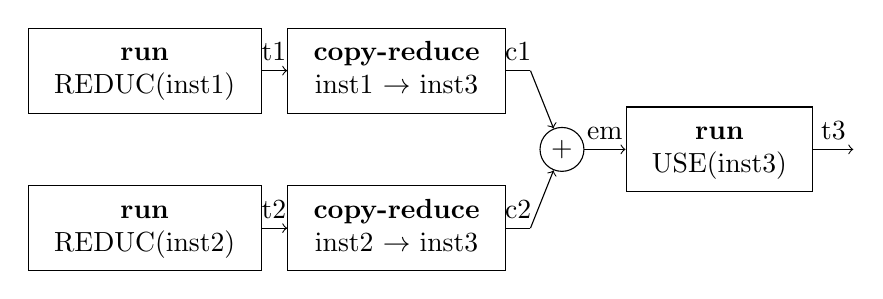
\begin{tikzpicture}
  %\path (1,3) node (t1) [shape=rectangle,draw] {run TASK\_A} -- node [right=1pt] {ea} +(0,-0.5) node[auto] {eax};
  \node (t1) at (0,1) [shape=rectangle,draw] {\begin{tabular}{c}{\bf run}\\REDUC(inst1)\end{tabular}};
  \draw (t1) to node[auto] {t1} (1.8,1);

  \node (t2) at (0,-1) [shape=rectangle,draw] {\begin{tabular}{c}{\bf run}\\REDUC(inst2)\end{tabular}};
  \draw (t2) to node[auto] {t2} (1.8,-1);

  \node (t3) at (3.2,1) [shape=rectangle,draw] {\begin{tabular}{c}{\bf copy-reduce}\\inst1 $\rightarrow$ inst3\end{tabular}};
  \draw (t3) to node[auto] {c1} (4.9,1);
  \draw [->] (1.8,1) to (t3.west);

  \node (t4) at (3.2,-1) [shape=rectangle,draw] {\begin{tabular}{c}{\bf copy-reduce}\\inst2 $\rightarrow$ inst3\end{tabular}};
  \draw (t4) to node[auto] {c2} (4.9,-1);
  \draw [->] (1.8,-1) to (t4.west);

  \node (t4j) at (5.3,0) [shape=circle,inner sep=2pt,draw] {+};
  \draw (t4j) to node[auto] {em} (6.1,0);
  \draw [->] (4.9,1) to (t4j);
  \draw [->] (4.9,-1) to (t4j);

  \node (t5) at (7.3,0) [shape=rectangle,draw] {\begin{tabular}{c}{\bf run}\\USE(inst3)\end{tabular}};
  \draw [->] (t5) to node[auto] {t3} (9,0);
  \draw [->] (6.1,0) to (t5.west);

\end{tikzpicture}
}
}
  %\vspace{-6mm}
  \caption{Reduction Example and Event Graph.\label{fig:reducevents}}
  \vspace{-4mm}
\end{figure}

Lines 39-61 of Figure~\ref{fig:runtimeapi} show a subset of the interface for physical regions.  
Each memory in the machine's memory hierarchy is named by a {\tt Memory} object (line 39).
The next object is a {\tt RegionMetaData} object (line 44), which defines a class of
regions.  Physical regions that belong to that class are created with the {\tt create\_instance}
method (line 51) and represented by {\tt RegionInstance} objects (line 56).  When creating a physical
region the client specifies the memory in which the physical region is going
to be allocated.  To maintain performance transparency, a new physical region can only be allocated
if the memory has sufficient capacity.
There is no automatic coherence of data between physical regions in the
same class.  It is the client's responsibility to manage data coherence using copies
between physical regions (line 59).  Like other operations copies can be
predicated on an event and return an event corresponding to completion.

If the only operations a task will perform on a region are reductions, a special reduction-only
instance can be created (line 52).  Rather than applying each reduction separately to the target instance,
the reduction operations can be accumulated in the reduction instance, and applied in bulk to 
the target using the {\em reduce\_to} operation (line 60).  This has several benefits.  First, it results
in much better performance, as we will show in section~\ref{subsec:reducmicro}), by reducing both
the total inter-node traffic and the overhead of that traffic while still allowing parallelism.
Second, a reduction-only instance is often smaller that the target instance, potentially improving
cache performance and helping address capacity issues for smaller memories (e.g. a GPU's device
memory).  For example, if reductions are being made to a single field in a larger structure, the 
reduction-only instance only needs to store that field and not the other fields that won't be 
modified by the reduction operation.

\texcomment{
If reductions are the only operations that will be performed on locations in a region instance,
a special reduction version can be created by providing the ID of a {\em reduction operator}
when the object is created (line 19).  Reduction-only region instances can 
increase the available parallelism and hide latency better, as we will show in 
section~\ref{subsec:reducmicro}.  The interface supports any reduction operation that
is commutative (i.e. multiple operations to the same location can be reordered without 
changing the final result) and is coded as an {\tt apply} method as shown on line 35.
Many commonly-used reduction operations are also {\em foldable} (e.g. $(l \text{ += } r_1) \text{ += } r_2$ can
be folded as $l \text{ += } r_1 + r_2$), and if the {\tt fold} operation and a {\em right identity}
(e.g. $0$ is a right identity for addition because $x + 0 = x$ for all $x$) are provided,
the runtime can use a {\em reduction fold instance}, described in section~\ref{subsec:reducimpl},
for even better performance.  Although the way they store data is very different,
reduction-only instances can be copied to other reduction-only instances (or normal 
instances) of the same class with the same asynchronous copy operations.  Copying between
instances with different layouts is only possible because physical regions provide 
the necessary information to understand the structure of the data.
}

%% Clients can also associate an operation as part of a physical region.  One example of
%% associating an operation with a physical region is shown on lines 13-14.  This instance
%% of the {\tt create\_instance} method
%% will create a physical region called a {\em reduction instance} that will be assoicated 
%% with the given {\tt ReductionOp} specified by the ID.  The interface for a {\tt ReductionOp} is shown on 
%% lines 26-33.  A reduction operation must have an {\tt apply} method, and can optionally 
%% implement two additional methods, {\tt init} and {\tt fold} that support additional 
%% optimizations described in Section~\ref{subsec:reducimpl}.  The two template parameters 
%% describe the base element type of the region ({\tt LHS}:left-hand-side) and the type of 
%% the argument to the reduction ({\tt RHS}:right-hand-side).  The reduction operation has 
%% total control over the choice of data layout for the reduction instance (not shown).
%% Reduction instances can be copied to other reduction instances with the same operation
%% or to regular physical regions of the same class.


An example using reduction-only regions is given in Figure~\ref{fig:reducevents} along with the resulting event graph.
Two reduction-only regions, {\tt inst1} and {\tt inst2}, are created in different memories to
be used with a reduction operation (lines 7-8).  (Reduction operations are registered at startup with integer IDs
as function pointers may not be portable across nodes.)  A physical region of the same class {\tt inst3}
is also created in a different memory (line 9).  Two tasks are launched that will apply
reductions locally into their respective reduction buffers (lines 10-11).  The resulting
events are then used to chain reduction copies back to {\tt inst3} after the tasks complete (lines 12-13).
The reduction operations accumulated in each of {\tt inst1} and {\tt inst2} are applied atomically
to {\tt inst3}.  The order in which the reduction operations are performed will be different from
the original order, but the requirement that reduction operations be commutative ensures the final
result is correct.  Finally, a merge on the events from the two reduction copies is 
performed and a final task using the results in {\tt inst3} is launched (lines 14-15).

%% SJT - redundant with first paragraph in this subsection?
%% Reductions and reduction instances illustrate only a single case where physical regions provide 
%% the structure necessary to conjoin an operation with data movement.  Physcal regions make our
%% interface easily extensible to arbitrary transformations and operations as a part of data movment.
%% While physical regions are a slightly higher-level construct than an annonymous
%% buffer of bits, we believe that the optimizations they enable are important in an asynchronous
%% environment.  Clients also still have access to an interface for controlling data layout through
%% the operations associated with physical regions which mitigates the loss in generality.

%{\em Physical regions} are the mechanism for reasoning about
%the placement and movement of data in the interface.  Physical regions are an 
%allocation of data in a single memory in the memory hierarchy.  Listing~\ref{lst:regionapi} 
%shows a subset of the physical region interface.  The first object in the interface
%is a {\tt RegionMetaData} object (line 1).  Region meta-data objects provide the interface for the
%creation of sets of physical regions that possess the same number and type of elements (but not necessarily
%the same data layout).  The interface is only able
%to copy data between two physical regions that were created by the
%same region meta-data object.  A runtime error will be generated if a copy is attempted
%between two physical regions that were not created by the same meta-data object.

%An instance of a physical region is represented by a {\tt RegionInstance} object (line 17).
%When creating a physical region the programmer must specify the {\tt Memory}
%in which the physical region is going to be allocated (line 10).  Memories are described
%in more detail in Section~\ref{subsec:machmodel}.  Once the physical region is created it
%cannot be moved.   There is no coherence of data between physical regions created by the 
%same meta-data object.  It is the programmer's responsiblity to manage data coherence
%using copies between physical regions (line 22-23).  Just like other operations,
%copies can be predicated on an event and return an event corresponding to
%completion.  
%A copy between two physical regions can only be performed if copies
%are permitted between the two memories where the regions were created.  
%The legality of copies can be discovered using queries to the {\tt Machine} object
%described in Section~\ref{subsec:machmodel}.

%The data held inside a physical region is accessed by another kind of object called an
%{\em accessor} (not shown).  Accessors support read, write, and reduction operations
%to elements inside the physical region.  Accessors can be specialized for the case where
%all memory is known to be directly accessible to the executing processor, which allows 
%for direct references to elements.  In cases where not all memory is directly accessable, 
%accessors supply the level of indirection necessary to convert operations into remote 
%memory operations (RMAs) if supported by the underlying hardware.  
%An example of this is described in more detail in Section~\ref{sec:impl}.

%One special (but common) case for applications is when reductions need to be performed.
%For reductions it is usually more efficient to store reduction
%operations in a local reduction buffer and then merge reduction buffers together at a later
%point in time.  To support this case the interface allows for the creation of a special kind
%of physical instance called a {\em reduction instance}.  The call to {\tt create\_instance} on
%lines 13-14 takes a {\em reduction operation} to be associated with a physical instance which
%tells the interface to create a reduction instance.  Reduction instances can only be accessed
%using a reduction of the given reduction type; any other accesses will result in a runtime
%error.  A reduction operation is a functor which must have at least one method of the type
%$(T_1 \rightarrow T_2 \rightarrow T_1)$ which takes a region element of type $T_1$ and a value
%to be reduced of type $T_2$ and creates and new region element.  Reduction operations can optionally 
%support two additional methods: a method that supplies an initial value of type $T_2$ and a 
%fold method of type $(T_2 \rightarrow T_2 \rightarrow T_2)$.  The presence of these methods
%enable additional optimizations for reductions described in Section~\ref{subsec:reducimpl}.

%Reduction instances can be copied using the same interface as regular physical instances.
%It is only legal to copy a reduction instance to a regular physical instance or another
%reduction instance of the same reduction operator.  Any attempt to copy from a regular physical 
%instance to a reduction instance will result in a runtime error.  A copy from a reduction 
%instance to a regular physical instance will apply all the reductions in the reduction 
%buffer to the physical instance.  If a copy is from one reduction instance to another, 
%the two reduction buffers will be merged.  The semantics of a merge are dependent upon 
%the underlying implementation of reduction buffers which is discussed in more detail 
%in Section~\ref{subsec:reducimpl}.




\subsection{Machine}
\label{subsec:machmodel}
The last component of the interface is the {\tt Machine} object, shown in lines 62-73 of Figure~\ref{fig:runtimeapi},
which provides initialization and run-time introspection
of the current machine.
The {\tt Machine} object is a singleton object that the client creates at the start of a
program, providing a task table that maps task IDs to function pointers,
and then invoking the {\tt run} method (lines 65).
Any running task can get a pointer to the machine object with the
{\tt get\_machine} method (line 67) and use it to obtain lists of all the {\tt Memory} (line 68) or 
{\tt Processor} (line 69) handles in the system.  Using the affinity methods (lines 71-72),
the application can also determine which memories are accessible by each
processor and with what performance, as well as which pairs of memories support copy operations.
%are able to efficiently copy data between themselves.

%% in the machine.
%% Second, the machine object provides an interface for the client to 
%% discover properties of the underlying machine (lines 35-43).  The machine object maintains
%% sets of all the unique {\tt Processor} and {\tt Memory} handles in the system.  Processors
%% were described in Section~\ref{subsec:procs}.  For every memory in the system there also 
%% exists a {\tt Memory} handle with a unique ID.  Different memories often, but not always, 
%% imply a different address space.  Examples of different memories are described in
%% Section~\ref{sec:impl}.

%For
%example, in a large cluster each node would have a different {\tt Memory} handle
%corresponding to each node's DRAM memory.
%However, if the cluster supported multiple GPUs then there would be a different
%{\tt Memory} handle for each GPU's {\em zero-copy} memory which shares part of the 
%address space with the corresponding node memory.  Memories will be used for describing
%the placement of data described in Section~\ref{subsec:phyreg}.

%The machine interface 
%contains three different object types: {\tt Processor} (line 1), {\tt Memory} (line 17), and a 
%singleton {\tt Machine} object (line 22).  For every processor (i.e. CPU core or GPU) in 
%the system there exists a {\tt Processor} handle with a unique ID naming that processor.  
%{\tt Processor} objects support a single {\tt spawn} operation (line 13-14) that will
%launch a {\em task} on that processor.   

%% The machine object also maintains two relations between the set of processors
%% and the set of memories:
%% \begin{itemize}
%% \item Processor-Memory: for each processor-memory pair whether
%% the processor can directly access (read and write) the memory and 
%% latency and bandwidth properties if access is possible
%% \item Memory-Memory: for every pair of memories whether copies can be
%% performed and latency and bandwidth properties if copies are possible
%% \end{itemize}
%%
%% The client can query these two relations by the {\tt get\_*\_affinity} calls
%% (lines 40-43) to discover properties of the machine.  

%These calls populate a vector with affinity structures (not shown)
%that contain latency and bandwidth information.  The programmer can restrict the query
%by specifying a specific processor or memory, otherwise information is returned
%about all processors and memories in the system.  





\section{Runtime Implementation}
\label{sec:impl}

There are currently two implementations of our interface:
one that works only on shared memory machines and another that
runs on large clusters with both CPUs and GPUs.  The shared-memory
implementation uses the POSIX threads library\cite{PTHREADS} (Pthreads)
and is primarily used for debugging.
The implementation for heterogeneous clusters uses Pthreads as 
well as the CUDA runtime library for GPUs\cite{CUDA} and the GASNet
API for large clusters\cite{GASNET07}.  

The heterogeneous implementation
models a cluster with CPUs and GPUs as having two kinds of processors 
and four kinds of memory.  Every CPU core is presented as a different {\tt CPU} processor
and every GPU is a {\tt GPU} processor.  This matches the scheduling granularity available
in the Pthreads and CUDA APIs respectively.  The first kind of memory is the 
system memory that is accessible by every CPU core on a given node.  The second is the 
framebuffer memory on each GPU (and accessible only by that GPU).  The third kind
of memory is system memory on a node that has been made accessible to the GPU(s) on
that node as well as the CPU cores, commonly referred to as {\em zero-copy memory}.
The final kind of memory is the portion of system memory on each node that has been registered with
the GASNet runtime to allow {\em remote memory access} (RMA) by other nodes in the cluster.
We refer to this memory as {\em GASNet memory}.
%% For every node in the system
%% there is a memory corresponding to the DRAM associated with that node.  For
%% every GPU in the system there are two memories corresponding to the framebuffer
%% memory and the zero-copy memory associated with that GPU \footnote{Zero-copy 
%% memory contains pages that are mapped in both framebuffer and node memory with
%% coherence maintained by the PCI-E protocol.}. The last memory is 
%% a global GASNet memory that represents pages that have been registered 
%% with all nodes in the system for supporting remote memory accesses (RMAs).
%% The GASNet memory provides the illusion of global memory.  CPU processors
%% can directly access their node memory, all zero-copy memories for GPUs on
%% their node, and the GASNet memory.  GPU processors can only access their
%% framebuffer memory and their zero-copy memory.  Copies are permitted
%% between all pairs of memory except between any framebuffer memory and
%% the GASNet memory.

In addition to the RMA capabilities, GASNet provides {\em active messages} for 
inter-node communication.  Active messages consist of a command and payload that
are sent by one node to another without any previous coordination.  Upon arrival
at a destination node, a handler routine is invoked to process the message.
%The handler may issue a response to the sender, but this is optional, and avoided
%as much as possible in our implementation due to the latencies involved in waiting
%for a response.  
One example of a case where we use active messages involves the {\tt spawn} call on a {\tt Processor}
object.  If the processor is not on the same node as the requestor, the information
%about the task (e.g. the task ID and arguments, the actual target {\tt Processor},
%the prerequisite event (if any), and the completion event ID) 
for the task is sent in an
active message to the node containing the target processor.  The recipient node
unpacks the message, and either places the task on the ready queue for the target
processor or marks it as being deferred until the prerequisite event has triggered.
%No response is sent to the original requestor.  The requestor already knows the event
%that corresponds to the completion of this task (since it was provided in the active
%message) - there is no utility in knowing exactly when the active message itself has
%been processed.

%% To support inter-node operations our implementation relies on GASNet active
%% messages for communication.  Active messages are a command and a payload
%% that are sent remotely and cause a handler to be run on the target node.
%% A simple example of our use of active messages can be illustrated by the 
%% {\tt spawn} call on a {\tt Processor} object.  Consider the case where {\tt spawn}
%% is invoked on a processor that is on a remote node.  This operation is converted into
%% an active message that contains all the information about the task launch.
%% When the active message is handled by the remote node, the task and all its
%% metadata are registered with the processor on which the task was launched.
%% While most of the implementation of our heterogeneous runtime is straight
%% forward, the next three sections describe in greater detail the nuances
%% of the implementation of events, locks, and reduction instances.

%% Our implementation uses a hierarchical model, in which data structures are shared by
%% all threads on the same node (taking advantage of the shared address space and low
%% latencies of using Pthreads mutexes and/or lock-free data structures).

%Due to space constraints, we will not cover every part of our implementation in
%detail, instead limiting our discussion to the three most interesting aspects:
%events, locks, and reduction instances.
Due to space constraints we cover only the most interesting parts of the implementation in detail.
We limit our discussion to three aspects:
events, locks, and reduction instances.

\subsection{Event Implementation}
\label{subsec:eventimpl}

Events are created on demand and are {\em owned} by the node on which they
were created.  The creation of an event occurs with no inter-node communication.
The space of event
handles is divided across the nodes at start-up time, allowing each node to assign handles
to new events without the risk of conflicting with another node's assignments.  The static division
of event handles also permits any node to determine the owning node of an event
without any communication.
%No broadcast of
%the event creation is required either, as the static division is sufficient to allow any
%node to correctly determine an event's owning node when (and only if) an operation on that
%event is performed on the other node.

%At event creation time, the owning node allocates a data structure to track the state of the event
%(i.e. triggered or not) as well as record a list of the operations that are known to be dependent
%on the event (e.g. initiation of a copy operation, placing a task on a processor's ready queue, waking
%up a waiting task).  However, the owning node only keeps a list of the dependent operations from the same
%node.  Every other node also allocates a corresponding data structure (the first time the event
%is referenced) to remember if the event has already triggered and to record its local dependent operations.
%Arbitrarily many dependent operations from a
%single node are aggregated into a single {\em event subscription} active message that is sent to the
%owning node.  The owning node keeps a bitmask of which other nodes have subscribed to the event, and when the
%event finally does trigger, a single {\em event trigger} active message is sent to each subscribing node,
%which notes that the event has triggered (in case queries come after the trigger) and executes the list
%of local operations that were dependent on that event.  (In the case that the triggering of the event has
%occurred before the reception of an event subscription, a trigger message is sent immediatel to the 
%new subscriber.)
When a new event is created, the owning node allocates a data structure to track the state of
the event ({\em triggered} or {\em untriggered}) as well as to record a list of dependent operations
(e.g. copy operation or task launch) from the same node called {\em waiters}.
The first operation dependent on an event
from a remote node will allocate the same data structure on the remote node.  A single
{\em event subscription} active message is then sent from the remote node to the owning node indicating
that the remote node should be informed when the event triggers.  Arbitrarily many dependent operations on
the remote node can then be added to the list of waiters without any additional communication.
When the event does trigger, the owner node notifies all local waiters and
sends a single {\em event trigger} active message to each node from which it has seen an event subscription
to notify remote waiters.
In the case where an event triggers while a subscription message is in flight from a remote node, the owner node will
immediately respond with a trigger message.

The actual triggering of an event may occur on any node.  If it occurs on a node other than the owning
node, an {\em event trigger} active message is sent from the triggering node back to the owning node, which
then forwards that message to all the other subscribed nodes.  The triggering node will automatically
notify its waiters and no message is sent from the owning node back to the triggering node.
%with the exception of the triggering node, which was
%able to execute its locally dependent operations (if any) immediately.  
While a remote trigger of an event can result in
the latency of a triggering operation being at least two active message flight times, it bounds the number of active
messages required per event to $2N-2$ where $N$ is the number of nodes 
%(which can be much smaller than the number of dependent operations) 
monitoring the event.  An alternative
would have been to share the list of subscribers so that the triggering node could notify all interested
nodes directly.  However, such an algorithm is both more complicated due to race conditions, and requires $O(N^2)$
active messages.  Any algorithm that is super-linear with the node count will not scale well, 
and as we will see in Section~\ref{subsec:eventmicro}, the latency of a single event trigger
active message is very small. 
%and any algorithm that is super-linear with the node count will not scale well.
%either is or will soon be an scalability issue for large systems.

The data structure used to track an event cannot be freed until all operations on that event have been
performed.  Creation and triggering can each happen only once, but there can be an arbitrary number of operations
that are dependent on an event.   Furthermore, some operations may not be requested until long after the
event has triggered.  Other systems incorporating events address this by reference counting event
handles\cite{Khronos:OpenCL}, but such reference counting adds both client and runtime overhead even when
limited to a single node; further overhead and complexity would be expected for a cluster-level
reference-counting approach.

%Instead of focusing on freeing event data structures, our implementation aggressively recycles them, 
%needing fewer total event data structures than a referencing counting implementation while also eliminating
%the overhead of reference counting.  The key observation is that one {\em generational event} data structure
% can efficiently capture the state of one {\em untriggered} event and a very large number (e.g. $2^{32}-1$)
%of already-triggered events.  An event's handle is expanded to include its generation number as well as the
%identifier for the underlying generational event.  In addition to the triggered-or-not state and list of
%dependent operations
%for the most recent generation, the owning node also remembers how many previous generations have already
%been triggered.  (There is no need to keep a list of dependent operations on previous generations.  Any
%new operation that is dependent on a generation that is known to be already triggered can immediately be
%executed.)  When an event is created, any generational event for whom the most recent generation has 
%triggered can be reused - the generation is increased by one and the state is returned to ``untriggered.''
%As before, this can be done with no inter-node communication.
Instead of attempting to free event data structures, our implementation aggressively recycles them.
Compared to a reference counting scheme our implementation requires fewer total event data structures
and has no client/runtime overhead.  The key observation is that one {\em generational event}
data structure can efficiently capture the state of one untriggered event and a very large 
number (e.g. $2^{32}-1$) of already-triggered events.  To accomplish this, we extend each event
handle to include its generation number as well as the identifier for its generational event.  Each
generational event remembers how many previous generations have already been triggered.  Any
new operation that is dependent on a generation that is known to already be triggered can immediately
be executed.  A generational event can be reused for a new generation as soon as the current generation has triggered. To
create a new event, a node finds a generational event in the triggered state,
increases the generation by one, and sets the generational event's state to untriggered.  As before, 
this can be done with no inter-node communication.

%A remote node's data structure is also efficient - the boolean values for whether the event
%has triggered and whether the event has already been subscribed to are replaced with the numbers of the most
%recent generation known to have triggered (this is received in the event trigger active message) and of the
%most recent generation the remote node has subscribed to (this is sent in the event subscription active
%message).  And as with the owner node's data structure, only
%one list of dependent operations is needed.  Although the latencies of a large system can delay the
%reception of an event trigger active message, if an operation is created that depends on a later generation
%of an event than what the current list of events is dependent on, that serves as a roundabout indication that
%the previous generation has indeed triggered, allowing the existing list of operations to be executed.
Nodes also maintain generational event data structures corresponding to remote events that they have
observed.  These data structures maintain the most recent known generation to have triggered as well
as the generation of the most recent subscription message sent (if any).  The distributed nature
of the system allows remote generational events to perform an interesting optimization.  If at any point a
remote generational event receives a request to wait on a later generation than its current
generation,
then it is safe to infer that all generations up to the requested generation have already 
been triggered because a new generation of the event was already created by the event's owner node.
All local waiters can then be notified even before receiving the event trigger message for the current generation.

Barriers are implemented as an extension of events.  In place of an event's triggered/untriggered state,
a barrier's owner tracks the number of outstanding arrivals.  When the arrival count 
reaches zero, the barrier is considered to have triggered.  Remote nodes send {\em barrier update}
active messages containing an adjustment value that is positive for {\tt alter\_arrival\_count} operations 
and negative for {\tt arrive} operations.  A simplified version of vector clocks\cite{Fidge1998} is used
to detect the race condition in which the barrier owner receives an {\tt arrive} operation before the
corresponding {\tt alter\_arrival\_count}.  When detected, the decrement of the count 
is delayed to avoid a spurious triggering of the barrier.

%% Events are created on demand by each node.  The ID of the creating node is encoded
%% in the upper bits of each event's ID and the creating node is said to be the 
%% event's {\em owner}.  If an event is used as an argument to an
%% operation on a remote node then the remote node can determine the owner of 
%% the event and send an active message to become a {\em subscriber} of the event.  When a
%% remote node becomes a subscriber to an event it guarantees that it will receive an active
%% message from the event's owner when the event triggers.  To minimize the amount
%% of communication that occurs between nodes, each node remembers the events to which it
%% is subscribed and guarantees that it only subscribes to an event once.  In the case
%% where there may be many remote waiters on an event 
%% this can dramatically reduce the number of inter-node active messages.

%% When an event triggers, it automatically notifies all of the operations that are waiting
%% on its local node.  The owner node will also send active messages to all of the subscriber nodes
%% telling them that the event has triggered.  Even though the event has now notified all of
%% its waiters, the memory on the owning node for storing the event cannot be reclaimed 
%% because there still may be handles to the event in the system which will request to
%% use this event in the future.  These requests will need to be satisfied saying that 
%% the event has already triggered for the duration of the application.  Rather than waste
%% the resources, we recycle event implementations.

%% A {\em dynamic event} is a logical construct that will only be triggered once and is the level
%% of abstraction at which the programmer reasons about events.  A {\em physical event} is an
%% actual event implementation that consumes resources on its owner node.  Multiple dynamic events
%% can be mapped to a single physical event.  However, for each physical event there can be at most
%% one {\em active} event in the set of dynamic events that are mapped to it.  An active event is a 
%% dynamic event that is yet to trigger.  By only having one active dyanmic event at a time 
%% there is no need to disambiguate event triggers that are sent to the physical event.  Each
%% physical event maintains a count of the number of trigger operations that it has observed.

%% When the runtime needs to return a handle corresponding to a new dynamic event, it finds
%% a physical event which currently has no active events (e.g. the trigger count equals the number
%% of dynamic events mapped to the physical event).  The runtime increases the count
%% of the number of dynamic events mapped to the physical event.  The handle that is returned 
%% corresponds to a new dynamic event which contains an ID that refers to the physical
%% event it is mapped to and a {\em generation} that is the dynamic event number for the particular
%% physical event.  Note that by definition the generation will always be one greater than the
%% trigger count at the time of dynamic event creation.

%% Within this framework it is now very easy to test whether the dynamic event specified by a
%% handle has triggered.  Using the ID that is contained within the handle we find the
%% physical event implementation (which may require an active message if the owner node is
%% remote from where the test is begin performed).  We can then compare the generation of
%% the handle to the number of observed triggers contained by the physical event.  If the
%% number of physical triggers is greater than or equal to the handle's generation, then
%% the dynamic event has triggered.  We show in Section~\ref{sec:apps} that in practice
%% the number of needed physical events is significantly less than the number of dynamic events.

%% We also leverage the mapping of dynamic events onto physical events to improve the efficiency
%% of subscriptions.  Nodes cache the last generation for every physical event for which they
%% have seen a trigger notification.  If the trigger test described above detects a trigger based
%% on the cached information then there would be no need for the subscription which would save an
%% active message.  If the event has not been detected to have
%% triggered locally then an active message is sent to the owner which would always have been necesary
%% without the dynamic to physical event mapping.

\subsection{Deferred Lock Implementation}
\label{subsec:lockimpl}

Like events, deferred locks, or locks from here on, are created on demand by the node on which the creation request was made.  The lock
handles are also statically divided across the nodes, allowing the creation to be done without inter-node
communication.  Whereas event ownership is static, locks may migrate; the {\em creating}
node is the initial owner, but that ownership can be transferred to other nodes.

Since any node may at some point be the owner of a lock, all nodes use the same data structure to track the
state of a lock on the node.
%(they differ only in when the structure is allocated -
%nodes other than the creator still wait until the first reference to the lock on that node).  
The structure tracks the following:
\begin{itemize} \itemsep1pt \parskip0pt \parsep0pt
\item {\em owner node} - the most recently known owner of the lock.  If the current node is the owner, this
information is always accurate.  If not, this information may be stale, but by induction the recorded 
owner is guaranteed to know the actual owner or the next node to query about ownership.
\item {\em lock status} - records whether the lock is currently held.  This is only valid if the node
is the current owner.
\item {\em local waiters} - a list of pending local lock requests.  This data is always valid on all nodes.
\item {\em remote waiters} - a bitmask of which other nodes have pending requests.  This bitmask is only
valid on the current owner.
\item {\em local payload pointer and size} - the local node's copy of the lock payload
\end{itemize}

When a lock request is made, an event is created to track when the grant occurs.  The current node then
examines its copy of the lock data structure to determine if it is the owner.
%(creating it if this the first operation for that lock on that node).  
If the current node is the owner and the lock isn't
held, the lock is granted immediately and the event is triggered.  If the lock is held, the event is added
to the list of local waiters.  Note that the event associated with
the lock request is the only data that must be stored.
%(This is the only thing that is stored.  The actual ``requestor'' of the lock
%is implicitly captured in which operations are dependent on the lock grant event.)  
If the current node isn't the owner, a {\em lock request} active message is
sent to the most recently known owner.  If the receiver of a lock request message is no
longer the owner, it forwards the message on to the node it has recorded as the owner.
%(If that information proves to be stale, the request is forwarded
%by the receiving node, eventually catching up to the current owner.)  
If the current owner's status shows
the lock is currently held, the bit for the requesting node is set in the remote waiters bitmask.  If the lock is
not held, the ownership of the lock is given to the requesting node via a {\em lock transfer} active
message.  A lock transfer message includes the bitmask of remote waiters and an up-to-date copy 
of the lock's payload.  The inclusion of the payload in the active message is the reason for the 
4KB size limit specified on payloads in Section~\ref{subsec:locks}.

Similarly, an unlock request is first checked against the local node's lock state.  If the local node is
not the owner, an {\em unlock} active message is sent to the most recently known owner, which is forwarded
if necessary.  Once the unlock request is on the lock's current owning node, the local waiter list is
examined.  If the list is non-empty, the lock remains in the locked state and the first lock grant
event is pulled off the local waiter list and triggered.  If instead the local waiter list is empty, the
lock state is changed to unlocked, and the bitmask of remote waiters is examined.  If there are any, then
one of them is chosen and the corresponding node becomes the new owner via a lock transfer active message.

The unfairness that results from a lock favoring local waiters over remote waiters is intentional.  When the
contention on a lock is high (the only time the question of fairness is relevant), the latencies
involved in transferring a lock between nodes can be the limiter on throughput.  By minimizing the number
of lock transfers, the throughput on the lock is maximized.  This effect will be demonstrated in
Section~\ref{subsec:lockmicro}.

\texcomment{
A similar issue can arise with the forwarding of lock request active messages.  If two nodes are
transferring a lock very quickly back and forth, a third node's request could be forwarded an arbitrary
number of times as it chases the lock around.  Although this can result in unfairness, it doesn't 
prevent forward progress.  A lock is only transferred to a node with at least one local waiter, so if 
the third node's request ever became the only one left, the lock transferring would stop and the request
would eventually catch up.
}

\subsection{Reduction Instances}
\label{subsec:reducimpl}

In addition to normal physical region instances, our implementation supports a special reduction-only
instance that differ in two important ways.  First, the per-element storage in a reduction-only instance
is sized to hold the ``right-hand side'' of the reduction operation (e.g. the $v$ in an operation like
$struct.field\ \text{+=}\ v$), allowing a more compact representation.  Second, individual reductions are applied
(atomically) to the local instance, which can then be sent as a large batched reduction to the target
instance.  When multiple reductions are made to the same element, they can be {\em folded} together locally,
further reducing the inter-node communication needed.  Note that the folding operation is not always
identical to the reduction operation itself.  For example, if the reduction operation is exponentiation,
the corresponding fold operation is multiplication, according to the following identity:
$$(r[i]\ \text{**=}\ a)\ \text{**=}\ b \quad \Leftrightarrow \quad r[i]\ \text{**=}\ (a * b).$$



\section{Benchmark Evaluation}
\label{sec:micro}

In this section we evaluate the heterogeneous implementation of our 
interface using several micro-benchmarks that test whether our implementation
approaches the underlying performance of the
hardware, and show that the optimizations described in Section~\ref{sec:impl}
are important.  All experiments were run on the Keeneland
supercomputer\cite{Keeneland}.  Each Keeneland node is composed of
two Xeon 5660 CPUs, three Tesla M2090 GPUs, and 24 GB of DRAM.  Nodes
are connected by an Infiniband QDR interconnect.

\subsection{Event Latency and Trigger Rates}
\label{subsec:eventmicro}
We implemented two micro-benchmarks for evaluating the performance of
events.  The first micro-benchmark tests the latency of event triggering,
both within a node and between nodes.  Processors are organized
into a ring and each processor in turn creates a user event that is dependent
on the previous processor's event.  The first event in this long chain of
dependent events is then triggered, and the time until the triggering of the
last event in the chain is measured.  The total time is divided by the number
of events in the chain to yield the mean trigger times.  In the single-node case, all events are local to
that node, so no active messages are required.  For all other cases, the
ring uses only a single processor per node so that every trigger requires
the transmission (and reception) of an event trigger active message.

%% is constructed.  The experiment measures the time from the triggering
%% of the first event to the triggering of the last event.  In the one node
%% configuration there is only one processor and all events are local to the
%% node.  In all other cases, there is only one processor per node which
%% guarantees that all event triggers result in an active message.  
%% Table~\ref{tab:eventlat} shows the results for both configurations.

\begin{figure}
\begin{center}
{ \small
\begin{tabular}{m{2cm}|c|c|c|c|c}
Nodes & 1 & 2 & 4 & 8 & 16 \\ \hline
Mean Trigger Time ($\mu$s) & 0.329 & 3.259 & 3.799 & 3.862 & 4.013 \\
\end{tabular}
}
\end{center}
\vspace{-6mm}
\caption{Event Latency Results.\label{tab:eventlat}}
\vspace{-4mm}
\end{figure}

\hyphenation{GASNet}

The calculated mean trigger times are shown in Table~\ref{tab:eventlat}.
The cost of manipulating the data structures themselves and running dependent
operations is shown by the single-node case, which experienced an average
latency of only 329 nanoseconds.  The addition of nearly 3 microseconds when
going from one node to two can be attributed to the latency of a GASNet
active message - others have measured similar latencies\cite{GASNET06}.
The gradual increase in latency with increasing node count is likely 
related to the underlying point-to-point nature of Infiniband communication,
which requires GASNet to poll a separate connection for every other node in
the system.
%% In the single node case the latency of triggering an event is only 
%% 329 nano-seconds.  For the multi-node cases, the triggering time is
%% between 3-4 micro-seconds which is the same as the cost of GASNet
%% active messages on Infiniband\cite{GASNET07}.  The gradual increase in latency with
%% node count is because each node must poll all the Infiniband connections for other nodes.
%% This cost of performing event triggers is in entirely in the hardware and the underlying software stack.

Our second micro-benchmark for events measures the maximum rate at which events can
be triggered by our implementation.  Instead of a single chain, many parallel chains
are created.  Additionally, each step of the chain can consist of parameterized number
of events, each one dependent on all the events from the previous step of the chain.
This parameter is called the {\em fan-in/out factor}.  The events within each step of
a chain are distributed across the nodes.  Recall from Section~\ref{subsec:eventimpl}
that the aggregation of event subscriptions
will limit the number of event trigger active messages to one per node (per event trigger)
even when the fan-in/out factor exceeds the node count.

%% triggers.  This benchmark creates {\em levels} of events where every event at a level
%% corresponds to a merge of all of the events at the previous level.  The benchmark is therefore
%% characterized by the number events at each level called the fan-in/out factor.  
%% The events at each level are evenly distributed between the processors in the machine.
%% In the case of an $n$-node experiment, only $n-1$ active messages will be required 
%% per event trigger because the event subscription mechanism described in 
%% Section~\ref{subsec:eventimpl}.  Figure~\ref{fig:eventthroo} shows the event triggering
%% throughput versus total nodes for a range of fan-in/out factors.

\begin{figure}
\begin{center}
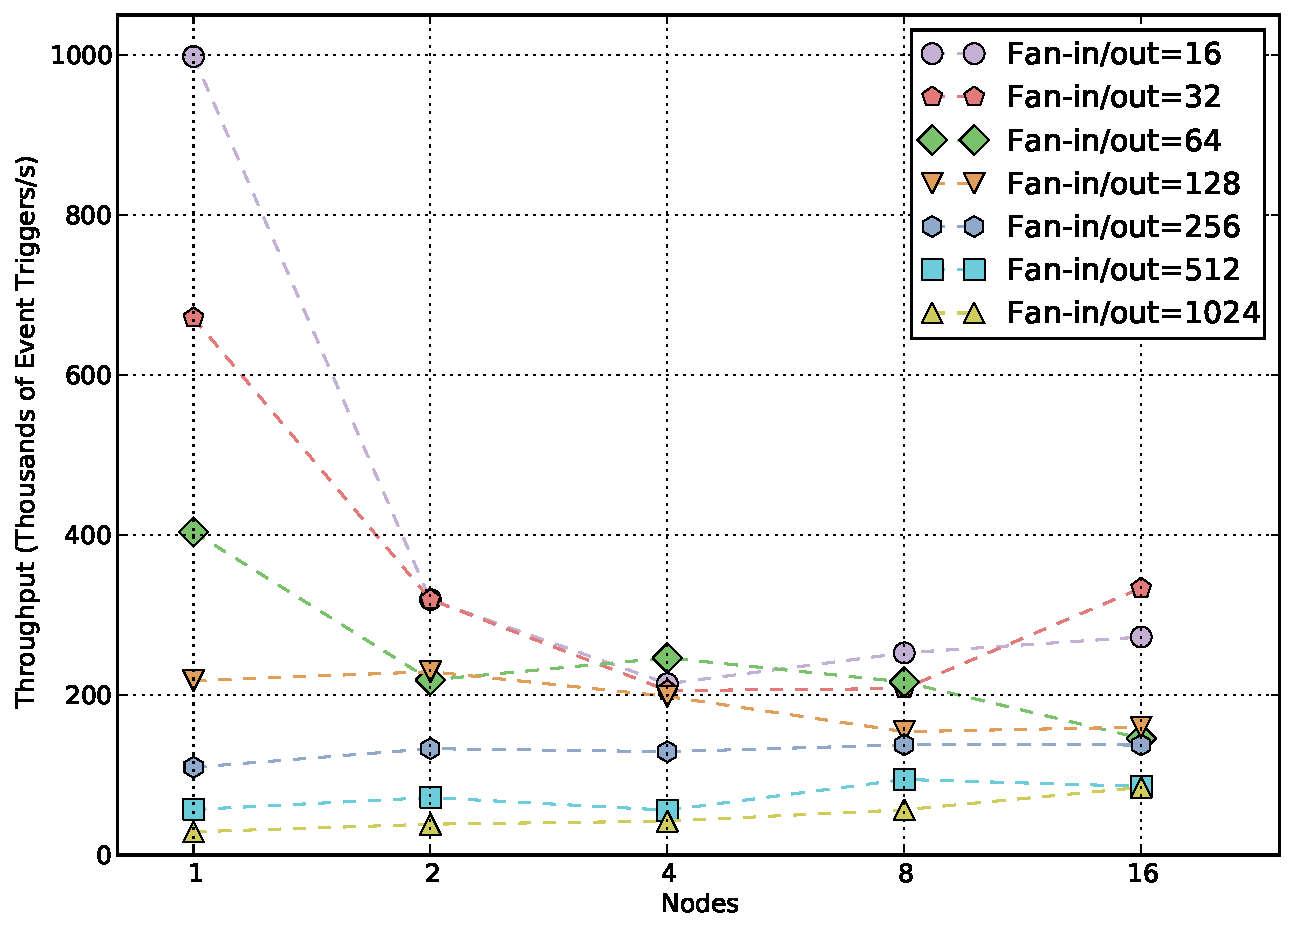
\includegraphics[scale=0.33]{figs/event_throughput.pdf}
\end{center}
\vspace{-6mm}
\caption{Event Trigger Rate Micro-Benchmark.\label{fig:eventthroo}}
\vspace{-4mm}
\end{figure}

Figure~\ref{fig:eventthroo} shows the event trigger rates achieved by our implementation
for a variety of node counts and fan-in/out factors.
For small fan-in/out factors, the total rate falls off initially going to two nodes as active
messages become necessary, but starts increasing slightly again at larger node counts.  Higher
fan-in/out factors require more messages and have lower throughput that also increases with
node count.  Although the number of events waiting on each node decreases with an increasing
node code, the minimal scaling indicates that the main bottleneck is in the processing of the
active message that each node must receive rather than the local redistribution of the triggering
notification.
%Note we can further improve performance by increasing
%the number of threads per node for handling active messages (in these experiments there
%is one per node), but in real applications these threads would consume hardware cores and
%take away computational resources from the primary application.  This is only a viable
%option for memory or communication bound programs.  

The compute-bound nature of the benchmark demonstrates that active messages do not tax 
the interconnection network and leave bandwidth available for application data movement.  
The event trigger rates achieved in this micro-benchmark are between one and two orders
of magnitude larger than the actual trigger rates required by the real applications
described in Section~\ref{sec:apps}.

\subsection{Lock Grant Rates}
\label{subsec:lockmicro}

Our lock micro-benchmark is designed to measure the rate at which locks can be granted.
A parameterized number of locks are created per node and their handles are made available to
every node.  Each node then creates a parameterized number of {\em chains} of lock/unlock
request pairs, where each request pair is to a random lock, and is made dependent on the 
previous lock/unlock pair's completion.  The chains are made long enough that startup
and cleanup times are negligible.  The total number of chains across all nodes gives the total
number of lock requests that can exist in the system at any given time.  All chains are
started at the same time (via a dependence on a single user event), and the total time to
process all the chains is divided into the total number of lock requests to yield and average
lock grant rate.

%% maximum throughput of lock
%% grants.  The benchmark is characterized by the number of nodes, the number
%% of locks initially created by each node, and the number of {\em chains} of
%% lock requests per node.  A chain is 1024 lock acquire and release operations that
%% are serialized by event dependences.  Each node creates the specified number of locks and
%% informs all other nodes of its lock handles.  All nodes create the specified number
%% of chains by randomly selecting from the set of all locks in the system.  All chains
%% are predicated on a user event.  The experiment measures the time from the triggering of
%% the user event to the completion of all chains.

Figure~\ref{fig:fixedlock} shows the lock grant rate for a variety of node counts and locks
per node.  The number of chains per node is varied so that the total number of chains in the system
is 1024 in all cases.  For the single-node cases, the insensitivity to the number of locks indicates
that the bottleneck is in the computational ability of the node to process the requests. 
For larger numbers of nodes, especially for the larger numbers of locks per node (where contention
for any given lock is low), the speedup with increasing node count suggests the limiting factor is
the rate at which lock-related active messages can be sent (nearly every request will require a
transfer of ownership).  Especially in the middle of the node count range, the performance actually
increases with
decreasing lock counts.  Although contention increases, the favoring of local lock requestors makes
this an advantage, reducing the number of lock-related active messages that must be sent.

%%  When going
%% from one node to two nodes, the bottleneck becomes the latency of transferring ownership of locks
%% between the nodes
%%  versus nodes in the system
%% for 256 total chains in the system.  Each line corresponds
%% to a different number of initial locks per node.  At small node counts, 
%% small numbers of locks per node cause high
%% contention and lock unfairness allows for very high throughput as many requests are
%% handled locally before locks are migrated.   When there are more total locks there
%% is lower contention and lower throughput because the ratio of lock grants to migrated
%% locks decreases.  At larger node counts, there are enough locks
%% in the system to remove contention and throughput improves.

\begin{figure}
\begin{center}
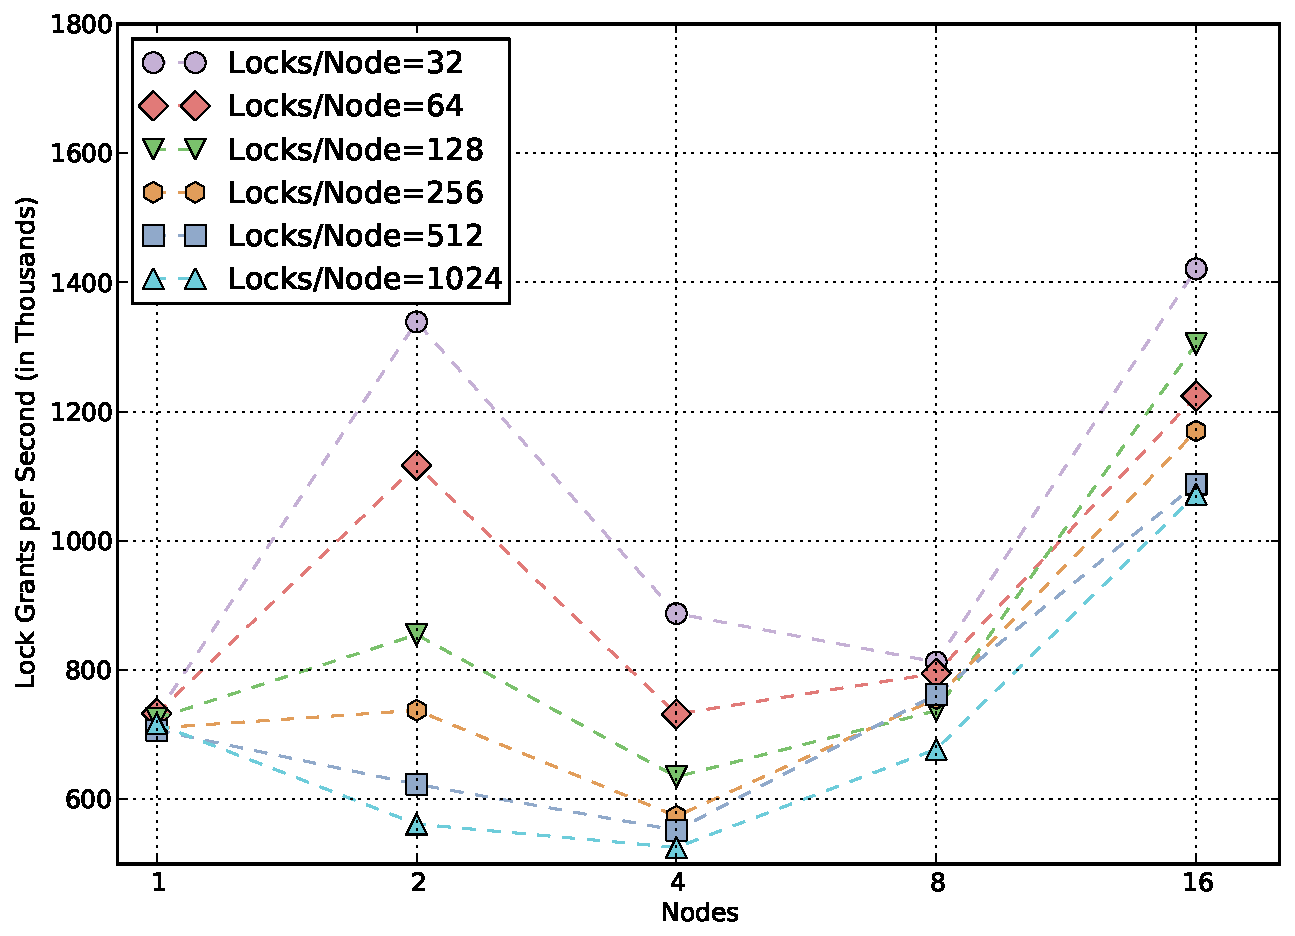
\includegraphics[scale=0.33]{figs/fixed_lock_chains.pdf}
\end{center}
\vspace{-6mm}
\caption{Lock Benchmark for Fixed Total Chains.\label{fig:fixedlock}}
\vspace{-4mm}
\end{figure}

To more clearly demonstrate the benefit of lock unfairness, even at large node counts, we show an alternative
cut of the experiment space in Figure~\ref{fig:fixednode}.
In this case the node count is fixed at 8 and lock grant rates are shown for a variety of total lock counts
and number of chains per node.
With only 32 chains per node (a total of 256 chains)
there is little contention and the grant rate is high.  As the number of chains per node increases there is
more contention for locks and the rate drops as a result.  For smaller lock counts, further increases in
the number of chains result in improved rates.  Note that the point on each line where this occurs
is when the chains per node is greater than total locks, which corresponds to the point where the expected 
number of requests per lock 
per node becomes more than one.  As soon as there are multiple expected requestors for the same lock on
a node, the unfairness property of our lock implementation is able to reduce the number of lock ownership 
transfers, yielding better performance.

\begin{figure}
\begin{center}
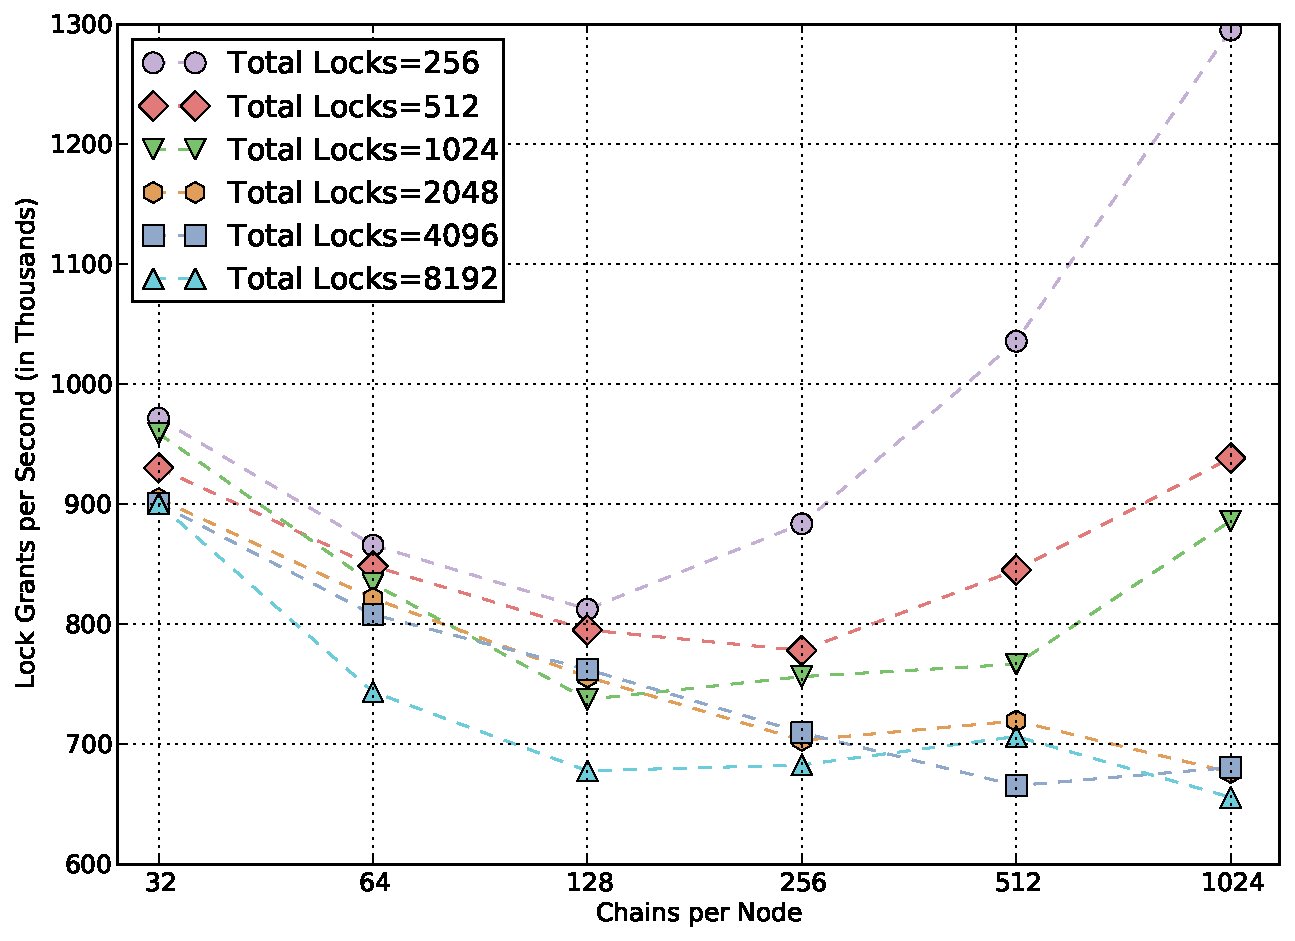
\includegraphics[scale=0.33]{figs/fixed_node_lock.pdf}
\end{center}
\vspace{-6mm}
\caption{Lock Benchmark for Fixed Node Count.\label{fig:fixednode}}
\vspace{-4mm}
\end{figure}


\subsection{Reduction Throughput}
\label{subsec:reducmicro}
To show the benefits of associating reduction instances we designed
a histogram micro-benchmark that requires all nodes to perform an addition reduction to a
physical region located in the globally visible GASNet memory (described in 
Section~\ref{sec:impl}).  Using the reduction interface described in Section~\ref{subsec:phyreg}
reductions are performed in five ways:

\begin{itemize} \itemsep1pt \parskip0pt \parsep0pt
\item Single Reads/Writes - Each node takes a lock on the global physical region and then for each reduction
reads a value from the physical region, performs the addition, and then writes the result back.  The lock is then released.
\item Single Reductions - Each reduction is individually sent as an active message to the node whose
system memory holds the target of the reduction.
\item Localized Instance - Each node takes a lock on the the global physical region, copies it to a new physical
region in its own system memory, performs all reductions to the localized region, copies the region back, and releases the lock.
\item Fold Instance - Each node creates a local fold reduction instance.
All reductions are folded into the instance, which is then copied back to the global region.
\item List Instance - Each node creates a local list reduction instance.
All reductions are appended to the list reduction instance, which is then copied back to the global region.
\end{itemize}

We ran two experiments, one corresponding with dense reductions and the other corresponding with sparse
reductions.  In each case a large random source of data is divided across into chunks, which are given to
separate reduction tasks.  There are 8 reduction tasks created for each node, one per processor.  The dense
case uses a histogram with 256K buckets and each reduction task performs 4M reductions.  The results for the
dense experiment are shown in Figure~\ref{fig:reducdense}.  The sparse case use a histogram with 4M buckets,
but only 64K reductions are performed by each task.  Results for the sparse case
be seen in Figure~\ref{fig:reducsparse}.

The dense experiment demonstrates that reduction fold regions perform 
best and scale well with the number of nodes, achieving over a billion reductions
per second in the 16 node case.  List regions also scale well, but perform about an
order of mangitude worse than folding regions in the dense case.  The use of a separate active message for
each reduction operation is another two orders of magnitude worse, demonstrating that data must be
transferred in larger blocks to be efficient on modern interconnect hardware.  The localized instance approach
works well for a single node, but its inherently serial nature doesn't benefit at all from increasing node counts.  Finally, the only time the latency of performing individual RMA reads and writes isn't disastrous is
on a single node (where the reads and writes are local).

The sparse case is very similar, except the scalability of the reduction fold case suffers from the
overhead of transferring a value for every bucket when most buckets are unmodified by a given task.
The reduction list case continues to scale well, surpassing the reduction fold performance at large
node counts.  This shows that
list regions are better suited for scaling sparse reduction operations.

\begin{figure}
\begin{center}
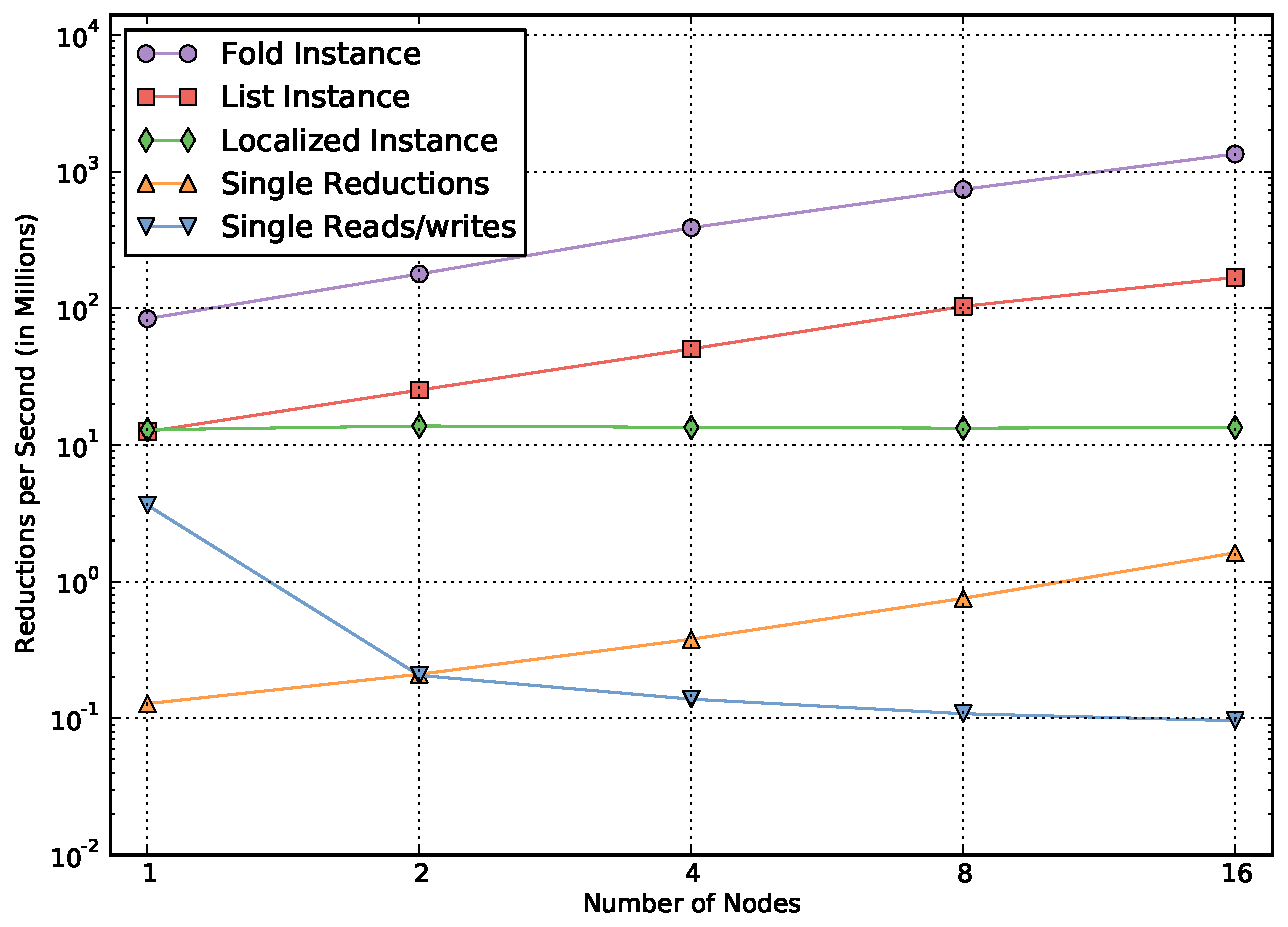
\includegraphics[scale=0.33]{figs/reduce_dense.pdf}
\end{center}
\vspace{-6mm}
\caption{Dense Reduction Benchmark.\label{fig:reducdense}}
\vspace{-4mm}
\end{figure}

\begin{figure}
\begin{center}
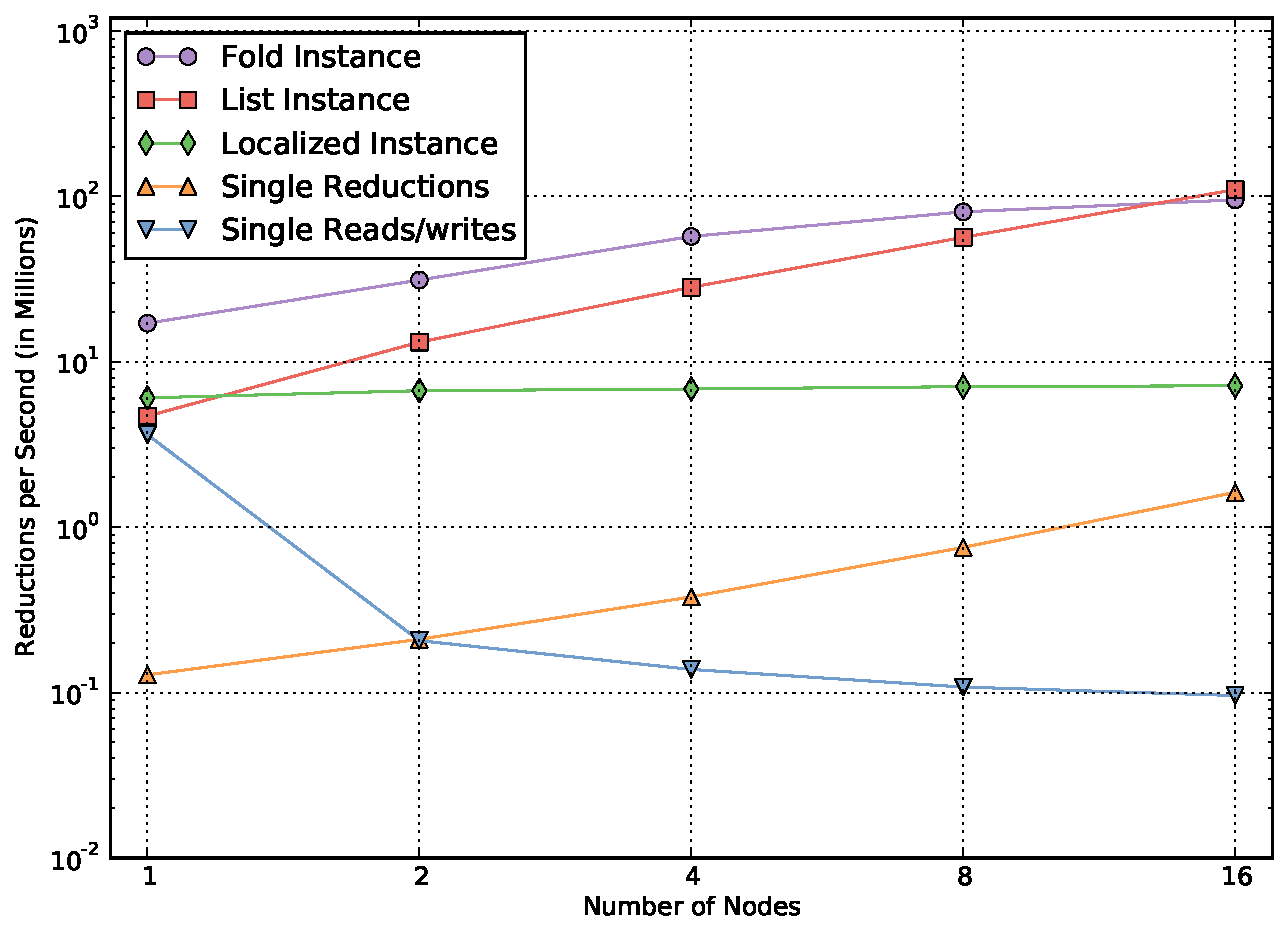
\includegraphics[scale=0.33]{figs/reduce_sparse.pdf}
\end{center}
\vspace{-6mm}
\caption{Sparse Reduction Benchmark.\label{fig:reducsparse}}
\vspace{-4mm}
\end{figure}



\section{Application Evaluation}
\label{sec:apps}
Legion is a high-level runtime system that has been implemented on top
of our interface\cite{Legion12}.  
%The Legion runtime is distributed so 
%that there is an independent scheduler for each processor in the machine.  
The Legion programming model is built around the abstraction of 
{\em logical regions} which express locality and independence properties 
of data.  Computation in Legion is organized into a tree of tasks where 
each task must specify which logical regions will be accessed.
When executing a Legion task, the Legion runtime receives requests
to execute sub-tasks along with their region requirements.
This stream of tasks with region requirements is analogous to a stream
of instructions with register requirements that are executed by 
a hardware processor.  Hardware out-of-order processors are designed to
run ahead of the actual execution of a stream of instructions
to ensure that the processor's pipeline is fully utilized.  Similarly, in a
Legion application, for every processor there is an instance of the Legion runtime
that takes a stream of tasks with region requirements and asynchronously
runs ahead of the actual execution using a scheduler called a {\em Software Out-of-Order Processor} 
(SOOP).  The SOOP leverages our interface by asynchronously issuing task launches, copy
operations, and synchronization operations with the dependencies between them expressed
as events.  The full details of the SOOP are beyond the scope of this paper
and are described in \cite{Legion12}.

The fully asynchronous design of the interface proposed in
this paper is crucial to Legion's SOOP implementation.  Without a fully
asynchronous interface, the SOOP would have to periodically invoke
blocking operations that would cause processors to stall and severely
limit Legion's ability to run ahead and keep the machine fully
occupied.  With a fully asynchronous interface the SOOP can hide latencies by 
running
far ahead of the actual execution, limited only by the physical resources
available in the machine, exactly like a hardware out-of-order processor.

In this section we demonstrate the performance properties of three
real-world applications that use the Legion runtime and the heterogeneous
implementation of our interface to run on the Keeneland supercomputer.
The three applications that we characterize are all multi-phase
applications that require parallel computation, data exchange, and
synchronization between phases. 

{\em Circuit} is a simulation of an integrated circuit that is described as an
irregular graph of components connected by wires.  The graph is partitioned
and distributed across the machine.  The computation for each time step consists
of three phases that calculate currents on the wires, distribute charge between
nodes, and update the voltages of all nodes.  In the distribute charge
phase, a single node may be updated by wires from multiple partitions.  Reduction instances 
are used to allow each partition to perform reductions in parallel and locally in GPU
framebuffer memory before merging all the reductions to a global instance
residing in GASNet memory.  Without reduction instances this phase
couldn't be performed using GPUs.

{\em Fluid} is an incompressible fluid flow simulation from the PARSEC
benchmark suite\cite{bienia11benchmarking}.  The original implementation can 
only be run on a single shared memory machine, but when written in Legion, Fluid can
be run on large distributed machines as well.  The Fluid simulation
models particles that flow through cells.  Each time step requires multiple phases
that update different properties of the particles contingent upon neighboring
particles in the same cell.  The space of cells is partitioned and neighboring
cells in different partitions must exchange data between phases.  Legion ensures
that these exchanges are done point-to-point by chaining copies and tasks
using events rather than employing a global bulk-synchronous approach.

{\em AMR} is an adaptive mesh refinement benchmark based on the third heat
equation example from the Berkeley Labs BoxLib project\cite{BoxLib}.  AMR
simulates the two dimensional heat diffusion equation using three different levels
of refinement.  Each level is partitioned and distributed across the machine.  Time steps require
both intra- and inter-level communication and synchronization.  Legion again
expresses dependences between tasks from the same and different levels through
events.

In Section~\ref{subsec:eventlife} we study the lifetime of events in
the Fluid application.  Section~\ref{subsec:lockmig} examines
the migration of locks in the Circuit application.  Finally, we demonstrate
that the asynchronous nature of our interface is essential to the
performance of Legion by comparing to bulk-synchronous
implementations of our target applications in Section~\ref{subsec:bulkcomp}.
  
\subsection{Event Lifetimes}
\label{subsec:eventlife}

We instrumented the heterogeneous implementation of our interface to 
capture event usage information.  Figure~\ref{fig:eventlife} shows
a timeline of the execution of the Fluid application on 16 nodes.
The dynamic events line measures the total number of event creations.
A large number of events are created - over 260,000 in less than 15
seconds - and allocating separate storage for every event would clearly
be difficult for long-running applications.  

Dynamic events are considered {\em live events} until their last operation 
(i.e. wait, trigger) has been performed.  The live events line
measures the number of events that are live at any given time.  After
the last operation on an event, a reference counting implementation would
be able to recover the storage associated with the event.  In this example 
a reference counting algorithm would reduce the storage needed for dynamic events
by over 10X, but could only do so at the cost of
computation and communication for performing the reference counting.  

As discussed in Section~\ref{subsec:eventimpl}, our implementation
requires storage that grows with the maximum number of {\em untriggered events}, a number
that is 10X smaller than even the maximal live event count.  The actual storage
requirements of our implementation are shown by the {\em physical events} line,
which is slightly larger than the peak number of untriggered events. 
The reason for this difference is because nodes create events locally if they have
no free generational events, even if there are unused generational events on remote nodes.
Despite this inefficiency, our implementation uses 5X less storage
than a reference counting implementation and avoids any overhead related to 
reference counting.  These savings would likely be even more dramatic for longer 
runs of the application, as the number of live events is steadily growing as the
application runs, while the peak number of generational events needed appears to 
occur during the start-up of the application.

%% much storage would be required for events using 

%%  about different kinds of events.  Figure~\ref{fig:eventlife} shows
%% the lifetimes of different types of events from a single run of the Fluid
%% application on 16 nodes using 8 processors per node.  Dynamic events 
%% is a monotonically increasing line that
%% corresponds to the total number of events created in the system.  By
%% the end of the run, the simulation created over 260,000 dynamic
%% events.  In contrast, the physical events line corresponds to the total number
%% of generational events required to represent the dynamic events 
%% across all the nodes in the system.  Less than 5,000
%% generational events were required to represent all the dynamic events
%% illustrating that the technique of mapping from dynamic events to generational 
%% events described in Section~\ref{subsec:eventimpl} was effective.

%% The live event line shows the total number of {\em live events} at a point in time.  Dynamic events
%% are considered {\em live events} until their last query has been performed.  The number of live
%% events is equivalent to the number of physical events that would be required
%% in a reference counted scheme.  In this case we see that by reusing
%% generational events, we require up to 4X fewer generational events than would be
%% required by a reference counted scheme.

%% In an ideal world the total number of generational events required would be
%% equivalent to the maximum number of generational events in the untriggered
%% state at any point.  The untriggered event line shows the number of generational
%% events in the untriggered state.  We see that the total number of generational
%% events is actually slightly higher than the maximum number of generational
%% events in the untriggered state at any point.  The reason for this is that unused
%% generational events cannot be shared across nodes, so in some cases nodes must
%% make new generational events eventhough there are unused generational events
%% on other nodes.  The small difference in these lines shows that in practice
%% this is only a minor inefficiency.

\begin{figure}
\begin{center}
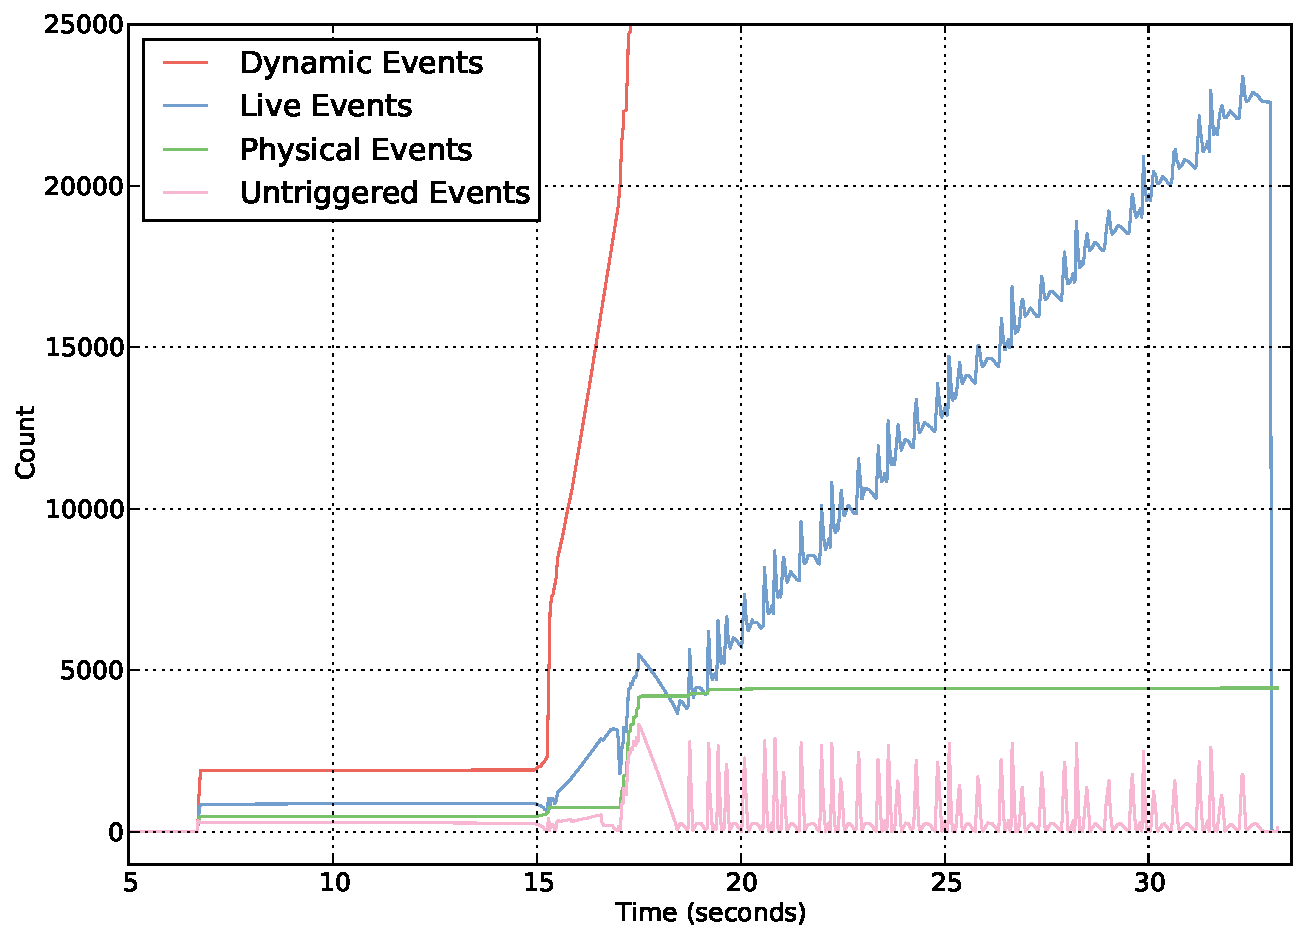
\includegraphics[scale=0.33]{figs/event_lifetimes.pdf}
\end{center}
\vspace{-6mm}
\caption{Event Lifetimes - Fluid Application.\label{fig:eventlife}}
\vspace{-4mm}
\end{figure}

%Figure~\ref{fig:eventlife} shows the event lifetimes in a run of the fluid application.  The total number
%of events created during the application is over 260,000.

\subsection{Lock Migration}
\label{subsec:lockmig}

We also instrumented our heterogeneous implementation to profile the usage of 
locks in real applications.  We measured how many locks were used in the application.  For
each lock we measured the number of lock requests and the number of times that the lock
had to be transferred from one node to another.  Figure~\ref{fig:lockcount} shows the results 
for the Circuit and AMR application, both running on 16 nodes.  The Circuit application uses
a larger number of locks (3336 vs. 1393), but most of them (86\%) are only used on the node on 
which they were created.  The AMR application exhibits more varied locking behavior, and in 
particular has locks that are requested more often than they are transferred.  Without the
ability for locks to migrate, these applications couldn't have made use of asynchronous
locks.

\begin{figure}
\centering

\subfigure[Circuit application]{
\label{fig:lockcount:ckt}
{
\renewcommand{\arraystretch}{1.2}
\small
\begin{tabular}{c|rrrrrrr}
\multicolumn{1}{l}{\multirow{2}{*}{{\renewcommand{\arraystretch}{1}\begin{tabular}{@{}l}\bf Lock\\\bf Xfers\end{tabular}}}}
& \multicolumn{7}{c}{\bf Total Lock Requests} \\
     & 
\multicolumn{1}{c}{\bf 0} &
\multicolumn{1}{c}{\bf 1} &
\multicolumn{1}{c}{\bf 2-8} &
\multicolumn{1}{c}{\bf 9-16} &
\multicolumn{1}{c}{\bf 17-32} &
\multicolumn{1}{c}{\bf 33-64} &
\multicolumn{1}{c}{\bf 65-128} \\
{\bf 0    } & 45 & 2611 & 9   & 26   & 79    & 78    & 30     \\
{\bf 1    } &  -  & 450  &  -   &   -   &   -    &    -   &  -      \\
{\bf 2-8  } &  - & - & - & - & - & - & -\\
{\bf 9-16 } &  -  &  -    &   -  & 8 & - & - & -\\
\end{tabular}
}}
\vspace{-2mm}
\subfigure[AMR application]{
{
\renewcommand{\arraystretch}{1.2}
\small
\begin{tabular}{c|rrrrrrr}
\multicolumn{1}{l}{\multirow{2}{*}{{\renewcommand{\arraystretch}{1}\begin{tabular}{@{}l}\bf Lock\\\bf Xfers\end{tabular}}}}
& \multicolumn{7}{c}{\bf Total Lock Requests} \\
     & 
\multicolumn{1}{c}{\bf 0} &
\multicolumn{1}{c}{\bf 1} &
\multicolumn{1}{c}{\bf 2} &
\multicolumn{1}{c}{\bf 3-4} &
\multicolumn{1}{c}{\bf 5-8} &
\multicolumn{1}{c}{\bf 9-16} &
\multicolumn{1}{c}{\bf 17-32} \\
{\bf 0   } & - & 94  & 592 & 414 & 94 & 3 & 41 \\
{\bf 1   } & - & 122 & -   & -   & -  & - & - \\
{\bf 2   } & - & -   & 6   & 7   & -  & - & - \\
{\bf 3-4 } & - & -   & -   & -   & 9  & 3 & - \\
{\bf 5-8 } & - & -   & -   & -   & -  & - & - \\
{\bf 9-16} & - & -   & -   & -   & -  & 7 & 1
\end{tabular}
}}
\vspace{-2mm}
\caption{Locks by Request and Transfer Counts.\label{fig:lockcount}}
\vspace{-4mm}
\end{figure}

%\subsection{Reduction Case Study}
%\label{subsec:reduccase}

%In this section we give a brief case study of how reductions make it possible
%to achieve high performance on a real application.  One of the three phases
%of the Circuit application involves reducing the current flowing in the wires

\subsection{Bulk-Synchronous Comparison}
\label{subsec:bulkcomp}

Our last set of experiments demonstrates that the asynchronous nature of our interface
is essential to the high performance of the Legion runtime system.  The Legion
implementations of our three applications have already been shown to outperform 
pre-existing implementations\cite{Legion12}.  To quantify the benefit of the asynchronous
nature of our interface, we implemented versions of our applications in
Legion in a bulk-synchronous style to compare against our existing implementations.  
These bulk-synchronous versions still run on top of 
the Legion runtime, but invoke blocking operations between computational phases,
communication phases, and synchronization.

Figure~\ref{fig:bulksync} compares
the performance of the bulk-synchronous implementations versus the original
implementations for Circuit, Fluid, and AMR respectively.  Each plot contains
performance curves for both implementations on two different problem sizes.
Circuit is a compute-bound application and the bulk-synchronous implementation
performs reasonably well.  By 16 nodes however the overhead grows to 19\%
and 22\% on the small and large inputs respectively.  The Fluid application 
has a more evenly balanced computation-to-communication ratio.  As a result,
Fluid performance suffers significantly more by switching to
a bulk-synchronous model.  At 16 nodes, performance is 135\% and 52\% worse
than the original Legion implementations on the small and large problem sizes
respectively.  Finally, the AMR application is a memory bound application, and on 16 nodes
the bulk-synchronous version is 82\% and 102\% slower on the small and
large problem sizes.

These results show that the asynchronous nature of our interface allows
the Legion runtime system to run ahead of actual execution which
provides significant latency hiding capability.  
The benefit of this latency hiding grows as the number of
nodes increases. % and as the computation-to-communication ratio decreases.
In all cases, the overhead of the bulk-synchronous
implementations grew with the node count.  As we continue to scale
applications to larger and larger machines, the ability of runtimes like Legion to run ahead
will be essential to hiding the large latencies inherent in such machine architectures.
The fully asynchronous nature of the interface presented in this paper
will be crucial for supporting this ability.


\begin{figure}[!ht]
\centering
\subfigure[Circuit Application]{
\label{fig:cktbulk}
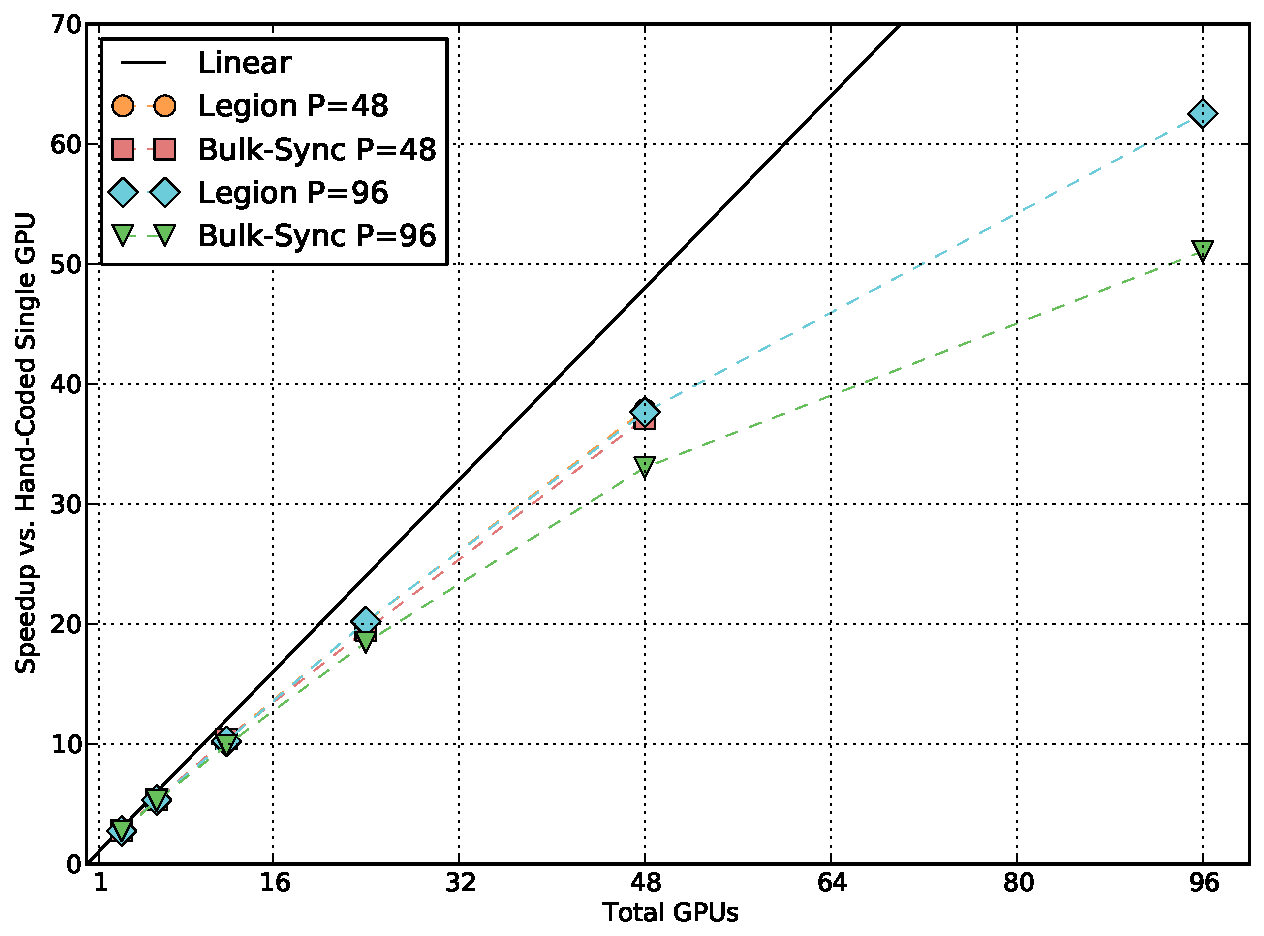
\includegraphics[scale=0.33]{figs/circuit_bulk_sync.pdf}
}

\subfigure[Fluid Application]{
\label{fig:fluidbulk}
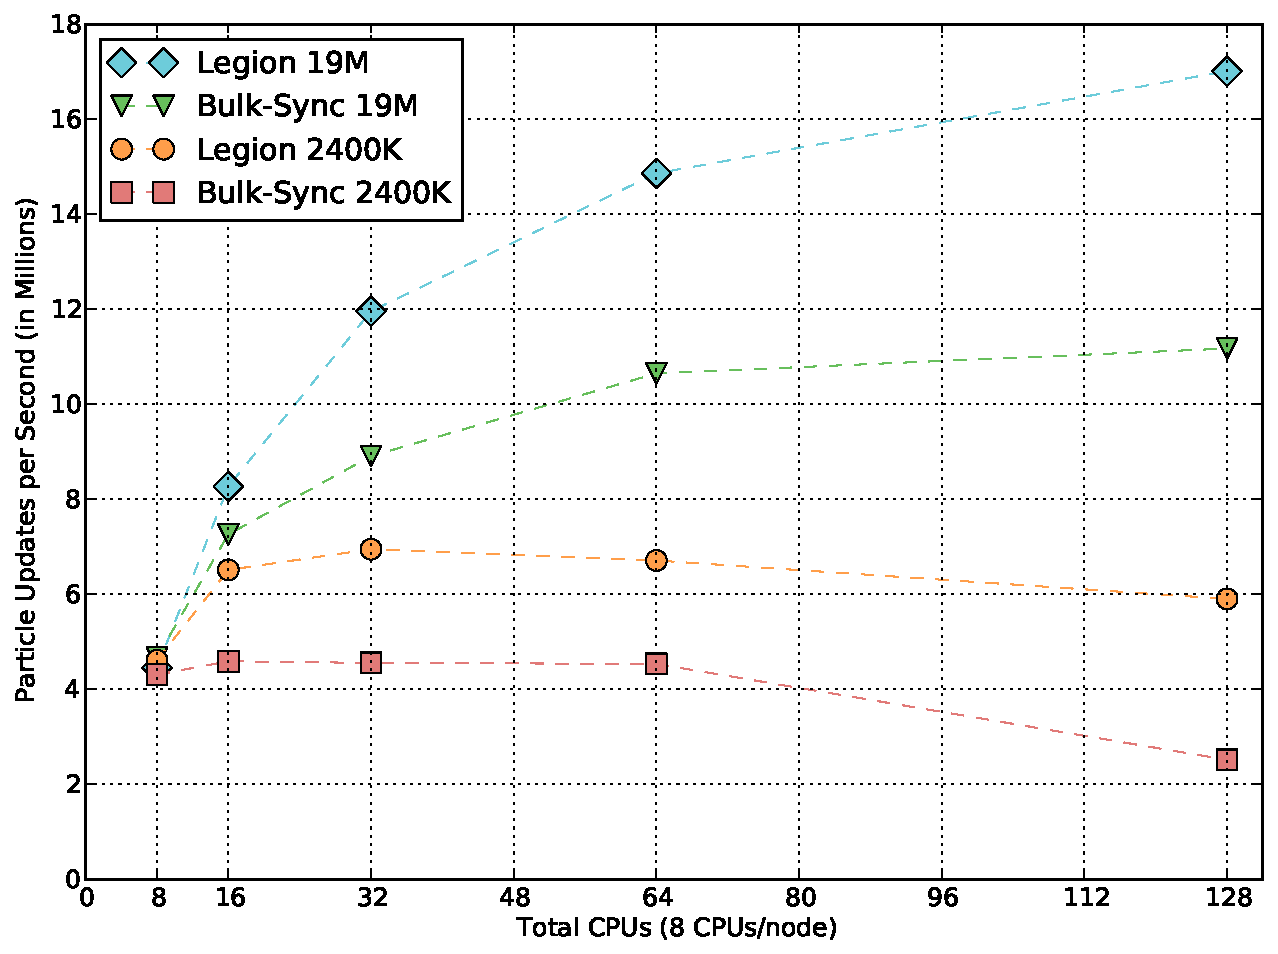
\includegraphics[scale=0.33]{figs/fluid_bulk_sync.pdf}
}

\subfigure[AMR Application]{
\label{fig:amrbulk}
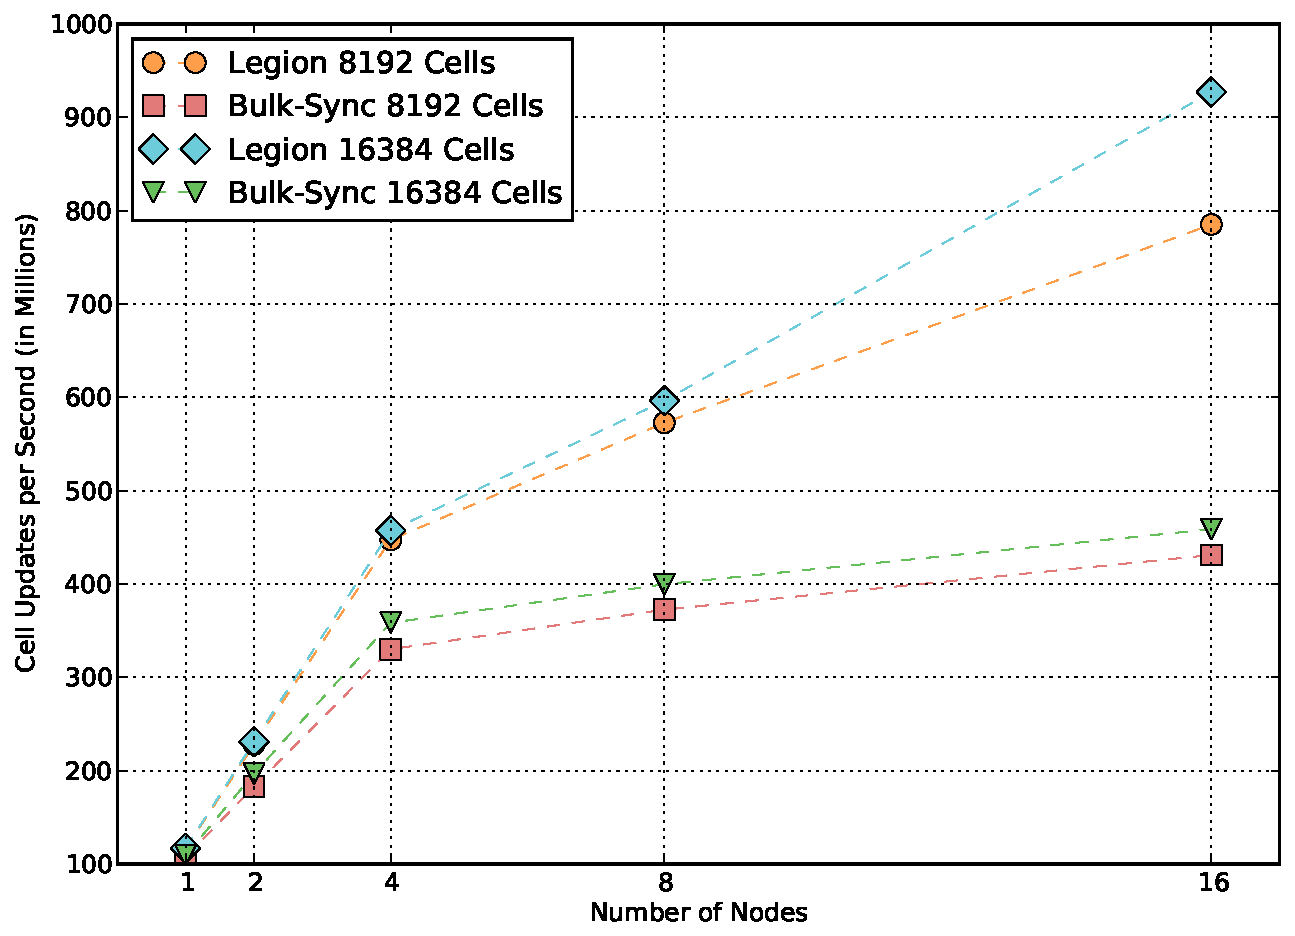
\includegraphics[scale=0.33]{figs/amr_bulk_sync.pdf}
}
\vspace{-4mm}
\caption{Bulk-Synchronous Performance.\label{fig:bulksync}}
\vspace{-4mm}
\end{figure}




\section{Related Work}
\label{sec:related}
Legion is most directly related to Sequoia \cite{Fatahalian06}.  Sequoia is array-based, with
a limited repetoire of ways to partition arrays.  Sequoia is a static language with a single unified hierarchy
of tasks and data; Legion is more dynamic with separate task and region hierarchies.

Deterministic Parallel Java (DPJ) is the only other region-based parallel system of which we are
aware\cite{Bocchino09}.  While there are similarities in the permission system and we have
reused some DPJ notation, there are differences stemming from DPJ's static approach.
Regions in Legion are first-class and can be created, partitioned, packed, and unpacked 
dynamically, allowing programmers to compute data organization at runtime; like Sequoia, DPJ
partition schemes must be statically decided.  Legion allows 
programmers to create multiple partitions of the same region to give different 
views onto the same data, which is not possible in DPJ.  
%DPJ only supports the 
%equivalent to Legion's exclusive and atomic coherence modes \cite{Bocchino11} 
%while Legion provides safe execution even in simultaneous environments.  
There is also a difference in emphasis: DPJ requires shared memory, while Legion 
is designed for distributed heterogenous machines.

Chapel \cite{Chamberlain:Chapel} and X10 \cite{X1005} also provide some Legion-like facilities.
Chapel's domains and X10's places provide the programmer with a 
mechanism for expressing locality, similar to regions in Legion.  However, domains
and places are not used for independence analysis to discover parallelism.
In contrast, Jade uses annotations to describe
data disjointness,  and like Legion leverages the disjointness information
to discover parallelism, but lacks a region system to name and organize unbounded collections of objects \cite{Rinard98}.  

% Unclear to me what subtleties need to be pointed out here and explained
% to properly differentiate our work
Many efforts use static region systems for  memory management (e.g., \cite{Tofte94, Grossman02}).
Our system is more closely affiliated with dynamic region systems used for expressing locality for performance \cite{Gay01}.

%In addition to region languages with static type systems, there have been several
%dynamic region languages.  Cyclone uses both a static type system and dynamic
%region checks to enforce memory safety properties of C programs\cite{Grossman02}.
%Gay and Aiken introduced RC which reference counts regions dynamically and uses
%a static type system to reason about effeciently garbage collecting regions\cite{Gay01}.

There have been many type and effect systems for ownership types
\cite{Boyapati03} including ones that leverage nested regions for describing
relationships \cite{Clarke02,Cameron07}.  However, ownership type and effect systems
are primarily used for reasoning about determinism in object oriented languages and
don't capture the range of disjointness properties that can be specified in Legion.

Reasoning about disjoint heap data is the strong suit of separation logic \cite{Reynolds02}.  
Concurrent separation logic\cite{Brookes04} has been 
used both to parallelize sequential programs\cite{Raza09,Gotsman07} and to provide 
a mechanism for reasoning about independence\cite{Hayman06}.
While we have borrowed some separation logic notation, we ultimately chose to use a 
permissions system as our primary formalism because separation logic does not easily
support reasoning about the interleaving of operations to non-disjoint regions of memory.

% I'm also not sure how much detail to go into here.  DPJ spends a lot of time
% on these papers, but I'm not sure I understand all the details of these papers.
% DPJ also cites Lu06 here, but I'm not sure if we have to
%Type and effect systems have also been used to reason about regions.  FX presented
%the original type and effect system on regions \cite{Lucassen88}, but was restricted 
%to using a finite number of regions and was incapable of describing nested data
%structures.  

% Do we need to enumerate what these disjointness properties are (DPJ does)
%Type and effect systems have also been used in the context of parallelism to discover
%deadlocks and race conditions \cite{Boyapati02,Abadi06,Jacobs08}, but do not present 
%any mechanism for discovering parallelism.

%Still not sure what we want to put here.
% DPJ sites additional separation logic papers but they didn't seem very similar.
% Let me know if you think we should include them as well.





\section{Conclusion}
We have presented Legion, a programming model and
type system for expressing locality and independence
to target heterogeneous, distributed parallel architectures.  
We implemented both a portable high-level and machine 
abstraction low-level runtime to support the Legion 
programming model.  Our implementation of Legion demonstrated
speedups up to 5.9X on a cluster of GPUs.


{
\small
\bibliographystyle{abbrv}
\bibliography{bibliography}
}

\end{document}


